%!TeX root=../apresentacao.tex
%("dica" para o editor de texto: este arquivo é parte de um documento maior)
% para saber mais: https://tex.stackexchange.com/q/78101/183146

% Apague as duas linhas abaixo (elas servem apenas para gerar um
% aviso no arquivo PDF quando não há nenhum dado a imprimir) e
% insira aqui o conteúdo do seu trabalho. Tome por base o
% arquivo corpo-apresentacao.tex do diretório conteudo-exemplo
% para a definição do título, autoria etc. e estrutura da
% apresentação.

\customtitlepage

% Slide com o qrcode
\showqrcode

\begin{frame}{Overview}
  \overview
\end{frame}

\section{Introduction}

%------------------------------------------------------------------------------
\begin{frame}{Context}
  \begin{itemize}
    \item Programmers use a tool named {\color{red}{compiler}} to generate binaries for their projects
    \begin{itemize}
      \item A {\color{red}{compiler}} is a program that translates code in language $A$ to another language $B$
      \item Remove the needs of coding in assembly
      \begin{itemize}
        \item Cheaper and faster software development
      \end{itemize}
    \end{itemize}
    \item Translation is done serially per file
    \begin{itemize}
      \item Parallel in the number of files
    \end{itemize}
  \end{itemize}
\end{frame}

%------------------------------------------------------------------------------

\begin{frame}{Context}
  \begin{itemize}
    \item Example: compiling a C file
  \end{itemize}
\begin{center}
\tikzstyle{block} = [rectangle, draw, fill=white,
    text width=6em, text centered, rounded corners, node distance=6.5cm, auto, minimum height=2em]
\tikzstyle{line} = [draw, -latex]
\tikzstyle{cloud} = [draw, ellipse,fill=white, node distance=2cm,
    minimum height=2em]
\scalebox{0.6}{
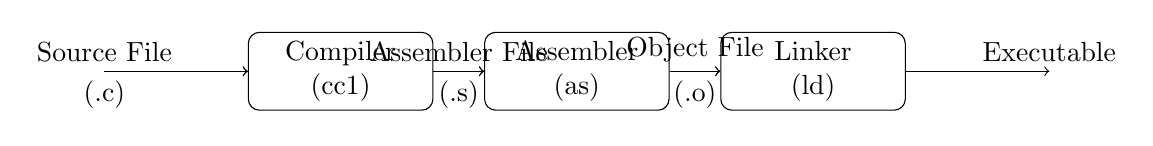
\begin{tikzpicture}[node distance = 3cm, auto]
    % Place nodes
    \node [block]                      (cc1) {Compiler \\ (cc1)};
    \node [block, right of = cc1]      (as) {Assembler\\(as)};
    \node [block, right of = as]       (ld) {Linker\\(ld)};
    \coordinate [left of=cc1]          (fonte);
    \coordinate [right of=ld]    (bin);

    % Draw edges
    \draw[->]    (cc1.east)    -- (as.west)       node[midway, above] {Assembler File};
    \draw[->]    (cc1.east)    -- (as.west)       node[midway, below] {(.s)};
    \draw[->]    (as.east)     -- (ld.west)       node[midway, above] {Object File};
    \draw[->]    (as.east)     -- (ld.west)       node[midway, below] {(.o)};
    \draw[->]    (fonte.west)  -- (cc1.west)      node[pos=0, above] {Source File};
    \draw[->]    (fonte.west)  -- (cc1.west)      node[pos=0, below] {(.c)};
    \draw[->]    (ld.east)     -- (bin.west)      node[pos=1, above] {Executable};
\end{tikzpicture}
}
\end{center}
\end{frame}

%------------------------------------------------------------------------------

\begin{frame}{Context}
  \begin{itemize}
    \item When combined with Makefiles, compilation works like this:
  \end{itemize}

\begin{center}
\tikzstyle{block} = [rectangle, draw, fill=white,
    text width=6em, text centered, rounded corners, node distance=1cm and 1.5cm, auto, minimum height=2em]
\tikzstyle{line} = [draw, -latex]
\tikzstyle{cloud} = [draw, ellipse,fill=white, node distance=2cm and 2cm,
    minimum height=2em, minimum width=2em]
\scalebox{0.6}{
\begin{tikzpicture}[node distance = 3cm, auto]
    % Place nodes
    \node [block]                         (make)   {Makefile};
    \coordinate[right=of make]            (c);
    \node [block, right=of make]          (fonte2) {source2.cpp};
    \node [block, above=of fonte2]        (fonte1) {source1.c};
    \node [block, below=of fonte2]        (fonte3) {fonte3.f90};

    \node [block, right=of fonte1]        (gcc)      {gcc};
    \node [block, right=of fonte2]        (g++)      {g++};
    \node [block, right=of fonte3]        (gfortran) {gfortran};

    \node [block, right=of gcc]           (objeto1) {object1.o};
    \node [block, right=of g++]           (objeto2) {object2.o};
    \node [block, right=of gfortran]      (objeto3) {object3.o};

    \node [block, right=of objeto2]       (ld) {ld};

    \node [block, below=of ld]            (bin) {Executable};

    % Draw edges
    \draw[->]    ([yshift=+0.7em] make.east)   -- (fonte1.west);
    \draw[->]    (make.east)                   -- (fonte2.west);
    \draw[->]    ([yshift=-0.7em] make.east)   -- (fonte3.west);

    \draw[->]    (fonte1.east)    -- (gcc.west);
    \draw[->]    (fonte2.east)   -- (g++.west);
    \draw[->]    (fonte3.east)   -- (gfortran.west);

    \draw[->]    (gcc.east)   -- (objeto1.west);
    \draw[->]    (g++.east)   -- (objeto2.west);
    \draw[->]    (gfortran.east)   -- (objeto3.west);

    \draw[->]    (objeto1.east)   -- ([yshift=+0.7em]ld.west);
    \draw[->]    (objeto2.east)   -- (ld.west);
    \draw[->]    (objeto3.east)   -- ([yshift=-0.7em]ld.west);

    \draw[->]    (ld.south)   -- (bin.north);


\end{tikzpicture}
}
\end{center}
\end{frame}

%----------------------------------------------------------------------------

\begin{frame}{Context}
  \begin{itemize}
    \item What happens if some files takes a really long time to compile?
    \begin{itemize}
        \item C++ blob files generated by other programs
        \item Heavy use of templates
    \end{itemize}
    \item Bottleneck in compilation!
  \end{itemize}
\end{frame}

%------------------------------------------------------------------------------

\begin{frame}{Context}
  \begin{itemize}
    \item Example: GCC compilation (64-threads Opteron machine):
  \end{itemize}

\begin{center}
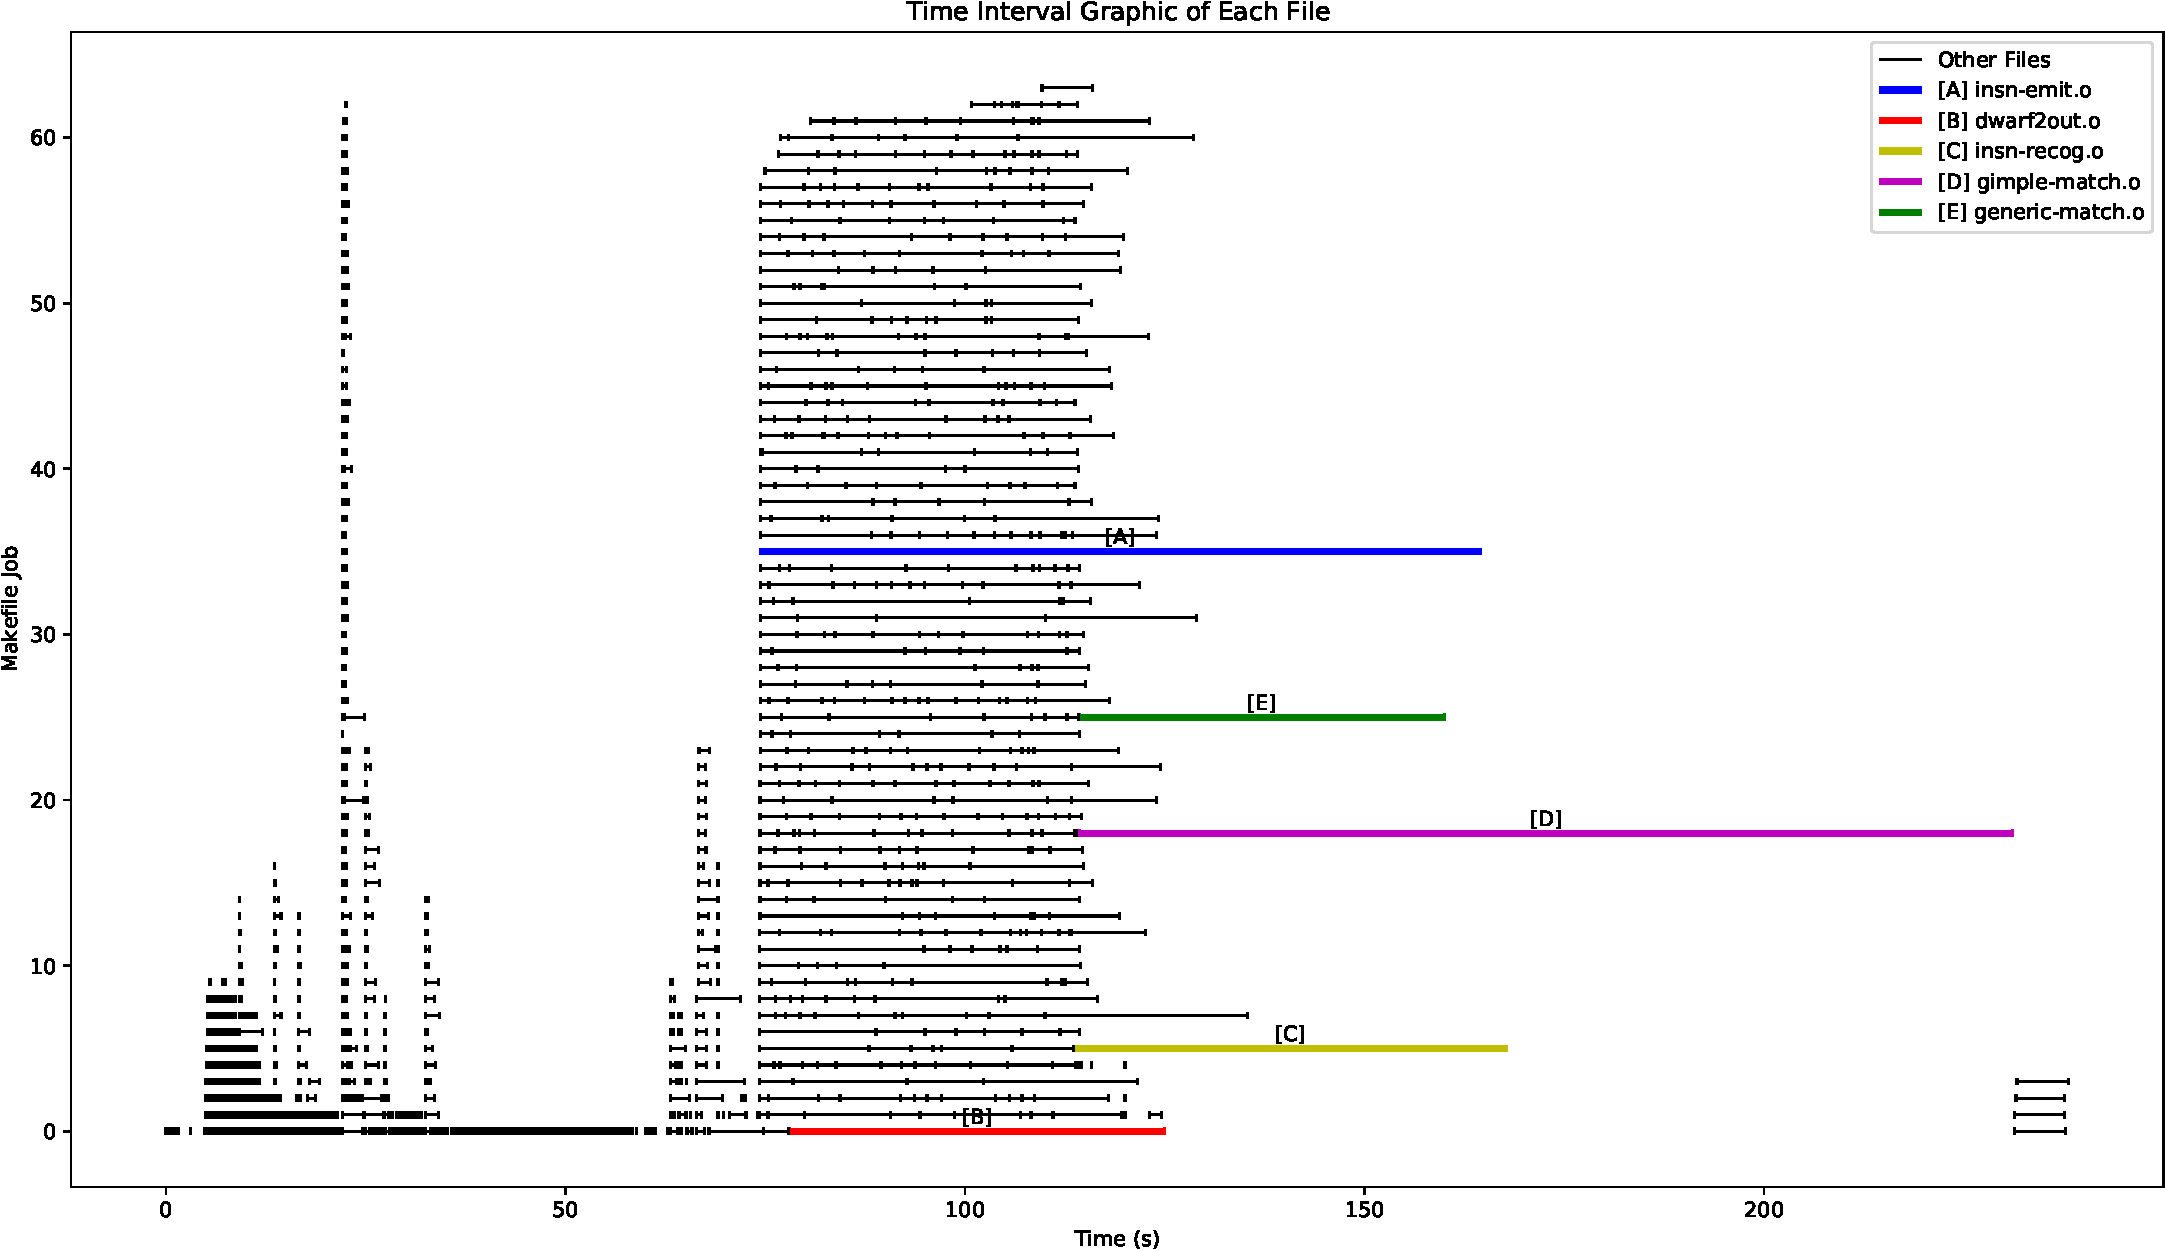
\includegraphics[width=0.8\paperwidth]{seq-crop.pdf}
\end{center}
\end{frame}

%------------------------------------------------------------------------------

\begin{frame}{Context}
  \begin{itemize}
    \item Example: GCC compilation (64-threads Opteron machine):
  \end{itemize}

\begin{center}
\includegraphics[width=0.8\paperwidth]{power-seq-crop.pdf}
\end{center}
\end{frame}

%------------------------------------------------------------------------------

\begin{frame}{Context}
  \begin{itemize}
    \item In the previous figure:
    \begin{itemize}
        \item Compilation is slow due to suboptimal use of CPU cores
    \end{itemize}
    \item Compilation consumes $19.659Wh$ of power
    \item[]
    \item Can we improve that by parallelizing the compiler?
  \end{itemize}

\end{frame}

%------------------------------------------------------------------------------

\begin{frame}{Context}
  \begin{itemize}
    \item Research Questions:
    \begin{itemize}
        \item \textbf{RQ1} - What is the main point in a compiler that can be improved with parallelism?
        \item \textbf{RQ2} - What is the performance improvement after parallelizing a compiler?
        \item \textbf{RQ3} - When compiling in parallel is faster than compiling sequentially?
        \item \textbf{RQ4} - How does a parallel compiler impact the power consumption?
    \end{itemize}
  \end{itemize}

\end{frame}

%------------------------------------------------------------------------------
\section{Theoretical Background}
%------------------------------------------------------------------------------
%------------------------------------------------------------------------------
\begin{frame}{Theorectical Background}
  \begin{coloredblock}{red!90!black}{Problems}
    \begin{itemize}
      \item Not every part of a compiler can be parallelized
      \begin{itemize}
        \item Parallelizing a industry standard compiler can be challenging
        \item Using only the code for ideas is not viable
      \end{itemize}
      \item Therefore, we must rely on compiler theory
      \begin{itemize}
          \item Can provide us strategies to parallelize on a compiler agnostic way
      \end{itemize}
      \item If theory says it is possible, it is a good option to try
    \end{itemize}
  \end{coloredblock}
\end{frame}
%------------------------------------------------------------------------------
\begin{frame}{Parser}
    \begin{itemize}
        \item Computer language programs are written in text files
        \begin{itemize}
            \item Needs to be \textit{parsed} to create an \textit{Abstract Tree} (AST) 
        \end{itemize}
        \item Parsing usually consists of two analyzers:
        \begin{itemize}
            \item Lexical Analyzer: break the input text into \textit{tokens}
            \item Syntactic Analyzer: read input tokens and try to reduce (or predict)
            to grammar rule
        \end{itemize}
    \end{itemize}
\end{frame}
%------------------------------------------------------------------------------
\subsection{Parser}
\begin{frame}{Parser}
\tikzstyle{block} = [rectangle, draw, fill=white,
    text width=6em, text centered, rounded corners, node distance=9cm, auto, minimum height=2em]
\tikzstyle{line} = [draw, -latex]
\tikzstyle{cloud} = [draw, ellipse,fill=white, node distance=2cm,
    minimum height=2em]

%TODO: Adcionar a tabela de símbolos aqui.
\begin{center}
\scalebox{0.7}{
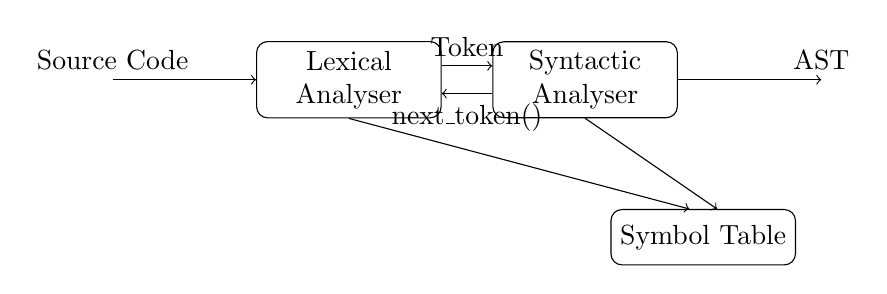
\begin{tikzpicture}[node distance = 3cm, auto]
    % Place nodes
    \node [block]                    (lexico) {Lexical Analyser};
    \node [block, right of = lexico] (sintatico) {Syntactic Analyser};
    \node [block] at (4.5, -2) (symtab) {Symbol Table};
    \coordinate [left of=lexico]     (fonte);
    \coordinate [right of=sintatico] (ast);

    % Draw edges
    \draw[->]    ([yshift=0.5em] lexico.east)       -- ([yshift=0.5em] sintatico.west) node[midway] {Token};
    \draw[->]    ([yshift=-0.5em] sintatico.west)   -- ([yshift=-0.5em] lexico.east)    node[midway] {next\_token()};
    \draw[->]    (fonte.west)                       -- (lexico.west)    node[pos=0, above] {Source Code};
    \draw[->]    (sintatico.east)                   -- (ast.west)   node[pos=1, above] {AST};
	\draw[->]    (sintatico.south)                  -- ([xshift=0.5em]symtab.north);
	\draw[->]    (lexico.south)                     -- ([xshift=-0.5em]symtab.north);

\end{tikzpicture}
}
\end{center}
\end{frame}

%------------------------------------------------------------------------------

\begin{frame}{Parser}
\begin{itemize}
    \item There are two general rules when parsing the input:
    \begin{itemize}
        \item Top-down Parsing: predict the input string from the starting rule $S$
        \item Bottom-up Parsing: reach the starting rule $S$ from the input string
    \end{itemize}
\end{itemize}
\end{frame}

%------------------------------------------------------------------------------

\begin{frame}{Parser}
\begin{itemize}
    \item With the following example grammar:
\begin{center}
\begin{align}
S &\rightarrow E \nonumber \\
E &\rightarrow T + E \; | \; T  \nonumber \\
T &\rightarrow a \times T \; | \; a \nonumber
\end{align}
\end{center}
    \item Input string: $a + a \times a$
    \item Top down parser:
    \begin{itemize}
        \item $ S \Rightarrow E \Rightarrow T + E \Rightarrow a + E \Rightarrow a + T \Rightarrow a + a \times T \Rightarrow a+ a \times a$
    \end{itemize}

\end{itemize}
\end{frame}

%------------------------------------------------------------------------------

\begin{frame}{Parser}
\begin{itemize}
    \item With the following example grammar:
\begin{center}
\begin{align}
S &\rightarrow E \nonumber \\
E &\rightarrow T + E \; | \; T  \nonumber \\
T &\rightarrow a \times T \; | \; a \nonumber
\end{align}
\end{center}
    \item Input string: $a + a \times a$
    \item Bottom up parser (bullet $\bullet$ denotes stack):
    \begin{itemize}
        \item $a + a \times a \Leftarrow T \bullet + a \times a \Leftarrow T + a \times a \bullet \Leftarrow T + a \times T \bullet \Leftarrow T + E \bullet \Leftarrow E \bullet \Leftarrow S \bullet$
    \end{itemize}
\end{itemize}
\end{frame}

%------------------------------------------------------------------------------

\begin{frame}{Parser}
\begin{itemize}
    \item After parsing is complete, an AST is generated
    \item This tree can be used for several analysis:
    \begin{itemize}
        \item Check for semantic errors in the code
        \item Find and Replace optimizations
        \item Calculating size of record type
        \item ... and so on
    \end{itemize}
\end{itemize}
\end{frame}

%------------------------------------------------------------------------------

\begin{frame}{Parser}
\begin{itemize}
    \item AST for the previous example:

\Tree[.S [.E [.T [\textit{a} ]][.E [$+$ ][.T [\textit{a} ][$\times$ ][.T [\textit{a} ]]]]]]

\end{itemize}
\end{frame}

%------------------------------------------------------------------------------
\subsection{Intraprocedural Analysis}
%------------------------------------------------------------------------------
%------------------------------------------------------------------------------
\begin{frame}{Three-Address Form (3AC)}
\begin{itemize}
    \item Expressions can become arbitrarly large \vspace*{-0.5cm}
    \begin{itemize}
        \item[] $$y = x \times x + x \times x$$ \vspace*{-0.3cm}
        \item Hard to simplify expressions
    \end{itemize}
    \item Idea: break expressions so that it have a maximum of two operands
    and one assignment \vspace*{-0.3cm}
    \begin{align}
          t_1 &= x \times x \nonumber \\
          t_2 &= x \times x \nonumber \\
            y &= t_1 + t_2 \nonumber
    \end{align} \vspace*{-0.6cm}
    \item Clearly, $t_1 = t_2$, so expression is $2x^2$
    \item Also useful on register allocation step
\end{itemize}
\end{frame}

%------------------------------------------------------------------------------

\begin{frame}{Control-Flow Graphs}
\begin{itemize}
    \item Program consists of more than a linear sequence of statements
    \begin{itemize}
        \item There are jumps, loops, comparisons, ...
    \end{itemize}
    \item This \textit{flow divergence} can be moduled using graphs
    \begin{itemize}
        \item Agglutinates a sequence of non-divergent statements in blocks (nodes)
        \item Edges show the possible path after the block is executed
    \end{itemize}
    \item Example:
\end{itemize}
\end{frame}

%------------------------------------------------------------------------------

\begin{frame}[fragile]{Control-Flow Graphs}

\begin{itemize}
    \item Example:
\end{itemize}

\begin{columns}[c]
      \begin{lstlisting}[
        language=pseudocode,
        style=pseudocode,
        style=wider,
        functions={},
        specialidentifiers={extern, call},
      ]
        function norm_1(x[n])
            sum := 0; i := 0
            while (i < n) {
                if (x[i] < 0)
                    sum -= x[i]
                else
                    sum += x[i]
                i := i + 1
            }
            return sum
        end
      \end{lstlisting}
\column{.5\textwidth}
    \begin{center}
    \scalebox{0.5}{
    \tikzstyle{line} = [draw, -latex]
    \tikzstyle{node} = [draw, rectangle]
    \begin{tikzpicture}[node distance = 2.3cm, minimum height = 1cm, auto]
        % Place nodes
        \node [node]                    (source) {$s_0$};
        \node [node, below of = source] (head) {while};
        \node [node, below of = head]   (check) {if};
        \coordinate[below of = check]            (c2);
        \node [node, left of = c2]  (true) {true};
        \node [node, right of = c2]   (false) {false};
        \node [node, below of = c2]   (merge) {$i \leftarrow i + 1$};
        \node [node, left of = head]   (return) {return};
        \coordinate[right of=false]    (c3);

        % Draw edges
        \draw[->]    (source)         -- (head);
        \draw[->]    (head)           -- (check);
        \draw[->]    (check)          -- (true);
        \draw[->]    (check)          -- (false);
        \draw[->]    (true)       -- (merge);
        \draw[->]    (false)      --  (merge);
        \draw    (merge.east) to [out=0, in=-90]  (c3);
        \draw[->]    (c3) to [out=90, in=0]  (head);

        \draw[->]    (head.west)  to [out=180, in=180] (return.east);
    \end{tikzpicture}
    }
    \end{center}
\end{columns}
\end{frame}

%------------------------------------------------------------------------------

\begin{frame}{Dataflow Analysis}
\begin{itemize}
    \item Analsyis need to propagate information about the program
    \begin{itemize}
        \item Example: \textit{liveness analysis}
        \item Find if variable will be needed in the future
    \end{itemize}
\end{itemize}
\end{frame}

%------------------------------------------------------------------------------

\begin{frame}{Dataflow Analysis}
\begin{itemize}
    \item \textit{Dataflow Analysis} is a framework to propagate information
    \begin{itemize}
        \item Runs on the Control-Flow Graph $G = (V, E, s_0, F)$.
        \item For each node $v$ in the graph, define a \textit{flow} function
              $f_v : \mathcal{L} \longrightarrow \mathcal{L}$
        \item Flow functions have the form (foward and backward):
    \end{itemize}
\end{itemize}

\begin{equation}\label{eq:forward}
	\texttt{in[} v \texttt{]} = \begin{cases}
	  BI,& \text{if } v = s_0 \\
	  \bigsqcap_{p \in \text{pred}(v)}f_p(\texttt{in[}p\texttt{]}) ,& \text{otherwise}
	\end{cases}
\end{equation}

\begin{equation}\label{eq:backward}
	\texttt{out[} v \texttt{]} = \begin{cases}
	  BI,& \text{if } v \in F \\
	  \bigsqcap_{p \in \text{succ}(v)}f_p(\texttt{out[}p\texttt{]}) ,& \text{otherwise}
	\end{cases}
\end{equation}

\end{frame}

%------------------------------------------------------------------------------

\begin{frame}[fragile]{Dataflow Analysis}

\begin{itemize}
    \item Example: Liveness Analysis
\end{itemize}

\begin{equation}\label{eq:liveness}
\begin{split}
	\texttt{in[} v \texttt{]} &= (\texttt{out[} v \texttt{]} - \texttt{kill[} v \texttt{]}) \cup \texttt{gen[} v \texttt{]} \\
	\texttt{out[} v \texttt{]} &= 
	\begin{cases}
	  \emptyset,& \text{if } v \in F \\
	  \bigcup_{p \in \text{succ}(v)}\texttt{in[}p\texttt{]} ,& \text{otherwise} \\
	\end{cases}
\end{split}
\end{equation}
\end{frame}

\begin{frame}[fragile]{Dataflow Analysis}

\begin{itemize}
    \item Example: Liveness Analysis
\end{itemize}

\begin{columns}[c]
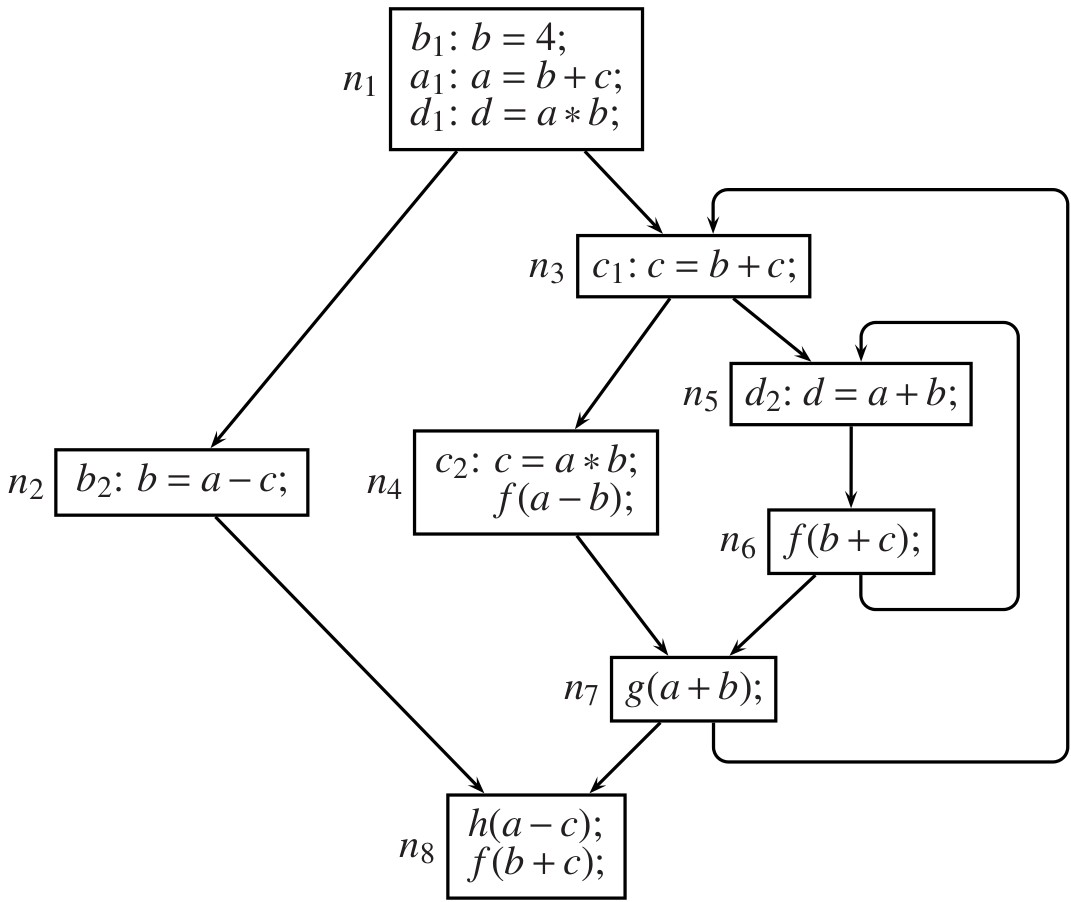
\includegraphics[scale=0.16]{cfg_liveness.png}

\column{.5\textwidth}

\vspace{-5.3cm}

\scalebox{0.55}{
\begin{tabular}{|c|c|c|c|c|c|c|}
\hline
\multirow{3}{*}{Vertex} & \multicolumn{2}{c|}{\multirow{2}{*}{Local Generation}}  & \multicolumn{4}{c|}{Global Information}                             \\ \cline{4-7} 
                        & \multicolumn{2}{c|}{}                                   & \multicolumn{2}{c|}{Iteration 1} & \multicolumn{2}{c|}{Iteration 2} \\ \cline{2-7} 
                        & $\texttt{gen[} n \texttt{]}$                        & $\texttt{kill[}n\texttt{]}$                   & $\texttt{out[}n\texttt{]}$             & $\texttt{in[} n\texttt{]}$             & $\texttt{out[}n\texttt{]}$             & $\texttt{in[} n\texttt{]}$            \\ \hline
$n_8$                   & $\{a, b, c\}$                & $\emptyset          $            & $\emptyset$               & $\{a, b, c\}$    & $\emptyset          $     & $\{a, b, c\}$    \\ \hline
$n_7$                   & $\{a, b\}$                   & $\emptyset          $            & $\{a, b, c\}$     & $\{a, b, c\}$    & $\{a, b, c\}$     & $\{a, b, c\}$    \\ \hline
$n_6$                   & $\{b, c\}$                   & $\emptyset          $            & $\{a, b, c\}$     & $\{a, b, c\}$    & $\{a, b, c\}$     & $\{a, b, c\}$    \\ \hline
$n_5$                   & $\{a, b\}$                   & $\{d\}      $            & $\{a, b, c\}$     & $\{a, b, c\}$    & $\{a, b, c\}$     & $\{a, b, c\}$    \\ \hline
$n_4$                   & $\{a, b\}$                   & $\{c\}      $            & $\{a, b, c\}$     & $\{a, b\}   $    & $\{a, b, c\}$     & $\{a, b\}   $    \\ \hline
$n_3$                   & $\{b, c\}$                   & $\{c\}      $            & $\{a, b, c\}$     & $\{a, b, c\}$    & $\{a, b, c\}$     & $\{a, b\}   $    \\ \hline
$n_2$                   & $\{a, c\}$                   & $\{b\}      $            & $\{a, b, c\}$     & $\{a, c\}   $    & $\{a, b, c\}$     & $\{a, c\}   $    \\ \hline
$n_1$                   & $\{c\}   $                   & $\{a, b, d\}$            & $\{a, b, c\}$     & $\{c\}      $    & $\{a, b, c\}$     & $\{c\}      $    \\ \hline

\end{tabular}
} %
\end{columns}

\end{frame}

%------------------------------------------------------------------------------

\begin{frame}{SSA form}
\begin{itemize}
    \item A variable can be redefined many times in a function
    \begin{itemize}
        \item Example: $x = 2$, and some lines after: $x = 42$
    \end{itemize}
    \item It can be refactored so variables can have one definition
    \begin{itemize}
        \item $x_1 = 2$, and then $x_2 = 42$
    \end{itemize}
    \item[]
    \item Advantage: easier analysis
\end{itemize}

\end{frame}

%------------------------------------------------------------------------------

\begin{frame}[fragile]{SSA form}
\begin{itemize}
    \item Example:
\end{itemize}

\begin{columns}[c]
        \begin{lstlisting}[
            language=pseudocode,
            style=pseudocode,
            style=wider,
            functions={},
            specialidentifiers={extern, call},
            ]
            if (condition) then
                a = -1;
            else
                a = 1;
            end
            u = a*v;
        \end{lstlisting}
\column{.4\textwidth}
        \begin{lstlisting}[
                language=pseudocode,
                style=pseudocode,
                style=wider,
                functions={},
                specialidentifiers={extern, call, PHI},
              ]
            if (condition) then
                $a_1$ = -1;
            else
                $a_2$ = 1;
            end
            $a_3$ = $\phi$($a_1$, $a_2$)
            u = $a_3$*v;
        \end{lstlisting}
\end{columns}
\end{frame}

%------------------------------------------------------------------------------

\begin{frame}[fragile]{SSA form}

\begin{itemize}
    \item Example:

\begin{align}
& x = 2 \nonumber \\
& y_1 = f(x) \nonumber \\
& y_2 = 1 \nonumber \\
& \texttt{return} \nonumber
\end{align}
    \item $y_2$ can be removed
    \begin{itemize}
        \item No use in the \textit{use-def} chain
    \end{itemize}

\end{itemize}
\end{frame}

%------------------------------------------------------------------------------

\begin{frame}[fragile]{Register Allocation}

\begin{itemize}
    \item Variables needs to be loaded in registers to perform operations
    \item Avoid unnecessary memory transfers
    \item Construct an interference graph and rename variables
\end{itemize}

\begin{columns}[c]
\column{.3\textwidth}
        \begin{lstlisting}[
            language=pseudocode,
            style=pseudocode,
            style=wider,
            functions={},
            specialidentifiers={extern, call},
            ]
			$a = b + c$
			$d = a * e$
			$f = d + 1$ 
        \end{lstlisting}
\column{.5\textwidth}
        \begin{lstlisting}[
                language=pseudocode,
                style=pseudocode,
                style=wider,
                functions={},
                specialidentifiers={extern, call, PHI},
              ]
			$r_1 = r_2 + r_3$
			$r_1 = r_1 * r_4$
			$r_1 = r_2 + 1$
        \end{lstlisting}
\end{columns}
\end{frame}

%------------------------------------------------------------------------------

\begin{frame}{Instruction Selection}

\begin{itemize}
    \item A single code can have multiple possible translations
    \begin{itemize}
        \item Example: $x = 0$ can be $\texttt{mov eax, 0}$ or $\texttt{xor eax, eax}$
    \end{itemize}
    \item Example: \textit{Macro Translation}
\end{itemize}

\tikzstyle{block} = [rectangle, draw, fill=white,
    text width=15em, text centered, rounded corners, node distance = 1cm and 1cm, auto, minimum height=2em]
\tikzstyle{line} = [draw, -latex]
\tikzstyle{cloud} = [draw, ellipse,fill=white, node distance=2cm,
    minimum height=2em]

\begin{center}
\scalebox{0.6}{
\begin{tikzpicture}
    % Place nodes
    \begin{scope}[node distance = 1cm and 5cm]
    \node [block]                  (c1) {$\textit{fib}_i = \textit{fib}_{i-1} + \textit{fib}_{i-2}$};
    \node [block, below=of c1]     (c2) {$\textit{fib}_{i-2} = \textit{fib}_{i-1}$};
    \node [block, below=of c2]     (c3) {$\textit{fib}_{i-1} = \textit{fib}_{i}$};
    \end{scope}

    \node [block, right=of c1]     (asm1) {\texttt{mov eax, DWORD [ebp-8]} \\ \texttt{mov ebx, DWORD [ebp-12]} \\ \texttt{add eax, ebx} \\ \texttt{mov [ebp-4], eax}  };
    \node [block, right=of c2]     (asm2) {\texttt{mov eax, DWORD [ebp-8]} \\ \texttt{mov [ebp-12], eax}};
    \node [block, right=of c3]     (asm3) {\texttt{mov eax, DWORD [ebp-4]} \\ \texttt{mov [ebp-8], eax}};

    % Draw edges
    \draw[->]    (c1.east)        -- (asm1.west);
    \draw[->]    (c2.east)        -- (asm2.west);
    \draw[->]    (c3.east)        -- (asm3.west);
\end{tikzpicture}
}
\end{center}

\end{frame}

%------------------------------------------------------------------------------

\begin{frame}{Instruction Selection}

\begin{itemize}
    \item Example: \textit{Tree Pattern Matching}
\end{itemize}
\begin{center}
	 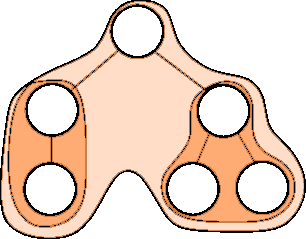
\includegraphics[scale=1.0]{tree_replace.pdf}
\end{center}

\end{frame}

%------------------------------------------------------------------------------

\subsection{Interprocedural Analysis}

%------------------------------------------------------------------------------

\begin{frame}{Interprocedural Analysis}

\begin{itemize}
    \item Programs consists of several functions
    \begin{itemize}
        \item Previous presented models only takes a single function in account
    \end{itemize}
    \item[]
    \item \textit{Callgraphs}: model interactions between functions
\end{itemize}

\end{frame}

%------------------------------------------------------------------------------

\begin{frame}{Callgraphs}

\begin{itemize}
    \item A \textit{callgraph} is a directed graph where:
    \begin{itemize}
        \item Nodes represent functions
        \item Edges represent call points
    \end{itemize}
    \item[]
    \item \textit{Callgraphs}: model interactions between functions
    \begin{itemize}
        \item Example:
    \end{itemize}
\end{itemize}

\begin{center}
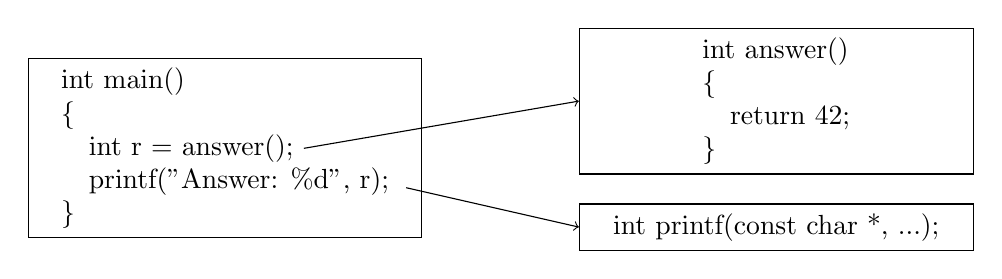
\begin{tikzpicture}[every text node part/.style={align=left}]
 \node [draw, minimum width=5cm] (main) { 
int main()\\
\{ \\
  \quad int r = answer(); \\
  \quad printf("Answer: \%d", r); \\
\}};
 \node [draw, minimum width=5cm] (resp) at (7, 0.6) {int answer()\\
 \{ \\
 \quad return 42; \\
 \}};
 \node [draw, minimum width=5cm] (printf) at (7, -1) {int printf(const char *, ...);};

 \draw[->] (1,0) -- (resp.west);
 \draw[->] (2.3,-0.5) -- (printf.west);
\end{tikzpicture}
\end{center}

\end{frame}

%------------------------------------------------

\begin{frame}[fragile]{Callgraphs}
\begin{itemize}
    \item Usually, only a \textit{summary} of the function is loaded in memory
    \begin{itemize}
        \item Reduce memory usage
        \item Example:
    \end{itemize}
\end{itemize}

\begin{center}
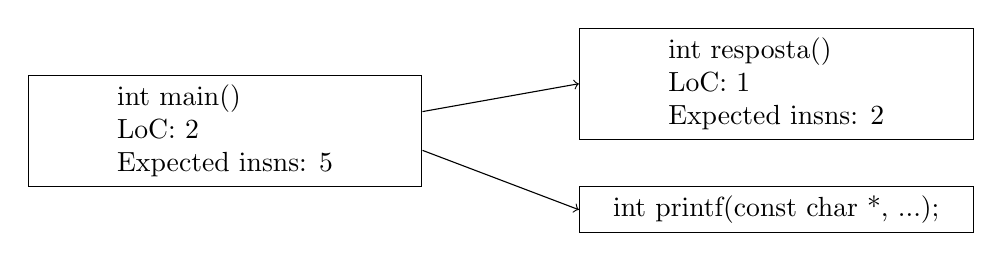
\begin{tikzpicture}[every text node part/.style={align=left}]
 \node [draw, minimum width=5cm] (main) {
int main()\\
LoC: 2 \\
Expected insns: 5
};
 \node [draw, minimum width=5cm] (resp) at (7, 0.6) {int resposta()\\
 LoC: 1\\
 Expected insns: 2
 };
 \node [draw, minimum width=5cm] (printf) at (7, -1) {int printf(const char *, ...);};

 \draw[->] ([yshift=+0.7em]main.east) -- (resp.west);
 \draw[->] ([yshift=-0.7em]main.east) -- (printf.west);
\end{tikzpicture}
\end{center}
\end{frame}

%------------------------------------------------------------------------------

\begin{frame}[fragile]{Callgraphs}
\begin{itemize}
    \item Classical interprocedural optimization: \textit{Function inlining}
    \begin{itemize}
        \item Copy \& paste the body of callee into caller
        \item Usually done when function is called once or is very small
    \end{itemize}
    \item Example: \textit{answer} will be inlined into main
\end{itemize}

\begin{center}
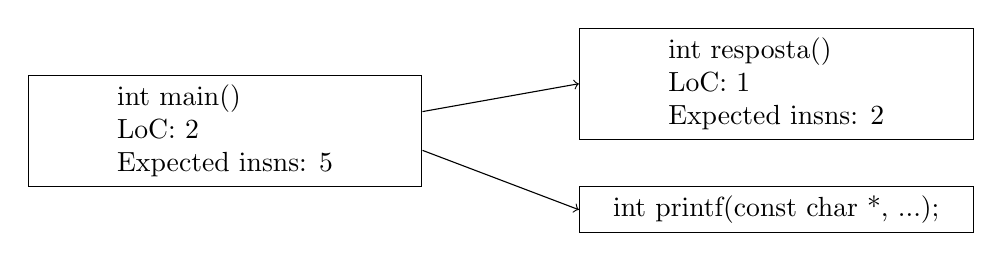
\begin{tikzpicture}[every text node part/.style={align=left}]
 \node [draw, minimum width=5cm] (main) {
int main()\\
LoC: 2 \\
Expected insns: 5
};
 \node [draw, minimum width=5cm] (resp) at (7, 0.6) {int resposta()\\
 LoC: 1\\
 Expected insns: 2
 };
 \node [draw, minimum width=5cm] (printf) at (7, -1) {int printf(const char *, ...);};

 \draw[->] ([yshift=+0.7em]main.east) -- (resp.west);
 \draw[->] ([yshift=-0.7em]main.east) -- (printf.west);
\end{tikzpicture}
\end{center}
\end{frame}

%------------------------------------------------------------------------------
\section{Related Works}
%------------------------------------------------------------------------------

\begin{frame}{Related Works}
\begin{itemize}
    \item \textit{Parallel Compilation} is not a new subject
    \begin{itemize}
        \item Previous authors have studied this subject before
        \item First papers dates from 1970
        \item Too much focus on \textit{parallel parsing}
    \end{itemize}
\end{itemize}
\end{frame}

\subsection{Parallel Parsing}

\begin{frame}{Parallel Parsing}
\begin{itemize}
    \item First work: Lincoln \cite{Lincoln:1970:PPT:987475.987478} and Krohn \cite{Krohn:1975:PAC:390015.808414}
    \begin{itemize}
        \item Splitting the input text
        \item Using vectorial units.
    \end{itemize}
\end{itemize}
\end{frame}

%--------------------------------------------------------------------------------

\begin{frame}{Parallel Parsing}
\begin{itemize}
    \item Fischer \cite{fischer1975parsing} and Mickunas \cite{Mickunas:1978:PCM:800127.804105}: Parallel LR$(k)$ parsing
    \begin{itemize}
        \item Split the input text into several parts
        \item Run a serial LR$(k)$ parser in each of then
        \item Heuristic to reconstruct the non-initial parser stack
        \item On failure, send tokens to the left-neighbor parser
    \end{itemize}
\end{itemize}
\end{frame}

%--------------------------------------------------------------------------------

\begin{frame}{Parallel Parsing}
\begin{itemize}
    \item Fowler and Paul \cite{fowler2009parallel} parallelized Earley and Packrat methods 
    \begin{itemize}
        \item Split the input text into several blocks
        \item Especulate new itens into the parser
        \item Run serial algorithm in each block
        \item[]
        \item Speedups: $5.5\times$ in Earley, and $2.5\times$ in Packrat
    \end{itemize}
\end{itemize}
\end{frame}

%--------------------------------------------------------------------------------

\begin{frame}{Parallel Parsing}
\begin{itemize}
    \item Barenghi \textit{et.al.} \cite{Barenghi:2015:PPM:2839536.2840146} proposes a parallel parser based on Operator Precedence Grammars
    \begin{itemize}
        \item Yacc-like generator
        \item[]
        \item Speedups: $5.5\times$
    \end{itemize}
\end{itemize}
\end{frame}

%--------------------------------------------------------------------------------
\subsection{Parallel Compilation}
%--------------------------------------------------------------------------------

\begin{frame}{Parallel Compilation}
\begin{itemize}
    \item Parallel compilation may include
    \begin{itemize}
        \item Parallel parsing
        \item Parallel code generation
        \item Parallel optimizations
    \end{itemize}
    \item[]

    \item Vandevoorde \cite{vandevoorde1988parallel} Parallelized a C compiler
    \begin{itemize}
        \item Syntatic analyiser pipelined with lexical analyser
        \item Compilation run in parallel in statement level
        \item[]
        \item Speedups: $10\%$ when pipelining the analysers, $3.1\times$ total in compiler
    \end{itemize}
\end{itemize}
\end{frame}

%--------------------------------------------------------------------------------

\begin{frame}{Parallel Compilation}
\begin{itemize}
    \item Wortman and Junkin \cite{wortman1992} Parallelized a Modula-2+ compiler
    \begin{itemize}
        \item Lexical Analyzer detect functions
        \item Symbol Table can handle not defined yet symbols
        \item Producer-consumer queue between Syntactic Analyser and Code Generator
        \item[]
        \item Speedups: Up to $6\times$
    \end{itemize}
\end{itemize}
\end{frame}

%--------------------------------------------------------------------------------

\begin{frame}{Parallel Compilation}
\begin{itemize}
    \item Lee and Ryder \cite{lee1994} proposed a parallel daftaflow analysis method
    \begin{itemize}
        \item Hybrid Algorithm: use both propagation and linear system techniques
        \item Graph is decomposed in stronggly connected partitions
        \item Each partition runs its dataflow analysis independently
        \item Local results are then propagated to other partitions
        \item Propagated results are propagated back to local nodes
        \item[]
        \item Speedups: Up to $7.8\times$
    \end{itemize}
\end{itemize}
\end{frame}

%--------------------------------------------------------------------------------

\begin{frame}{Parallel Compilation}
\begin{itemize}
    \item Kramer \textit{et al.} \cite{krammer1994combining} proposed another parallel daftaflow analysis method
    \begin{itemize}
        \item Convert the Graph into a DAG
        \item Proves that dataflow solutions to this DAG is equivalent to the original graph
        \item Process in parallel by levels
        \item[]
        \item Speedups: Up to $5.4\times$
    \end{itemize}
\end{itemize}
\end{frame}

%--------------------------------------------------------------------------------

\begin{frame}{Parallel Compilation}
\begin{itemize}
    \item Panchenko \textit{et al.} \cite{panchenko2021lightning} Present Lightning BOLT
    \begin{itemize}
        \item Reads generated binaries from other compilers
        \item Output optimized version of them
        \item Parallel passes:
        \begin{itemize}
            \item Control-Flow Graph construction
            \item Local Optimizations
            \item Identical Code Folding
            \item Shrink Wrapping
        \end{itemize}
        \item[]
        \item Speedups: Up to $5.4\times$
    \end{itemize}
\end{itemize}
\end{frame}

%--------------------------------------------------------------------------------
\subsection{Link Time Optimization}
%--------------------------------------------------------------------------------

\begin{frame}[fragile]{Link Time Optimization (LTO)}
\begin{itemize}
    \item \textit{Classical Compilation Method}: each file is compiled separately
    \begin{itemize}
        \item Side effect: no cross-module optimizations
        \item Example:
    \end{itemize}
\end{itemize}

  \begin{columns}[c] % The "c" option specifies centered vertical alignment while the "t" option is used for top vertical alignment

    \column{.45\textwidth} % Left column and width
    \begin{center}
        File a.c
    \end{center}

\begin{lstlisting}[
        language=pseudocode,
        style=pseudocode,
        style=wider,
        functions={},
        specialidentifiers={extern, call, var},
]
extern function answer();

function main()
  var r = answer();
  print("Resposta: ", r);
\end{lstlisting}

    \column{.5\textwidth} % Right column and width
    \begin{center}
        File b.c
    \end{center}

\begin{lstlisting}[
        language=pseudocode,
        style=pseudocode,
        style=wider,
        functions={},
        specialidentifiers={extern, call},
]
function answer()
  return 42;





\end{lstlisting}

  \end{columns}

\begin{itemize}
    \item Function \texttt{answer} can not be inlined into \texttt{main}
\end{itemize}

\end{frame}

%--------------------------------------------------------------------------------

\begin{frame}[fragile]{Link Time Optimization (LTO)}
\begin{itemize}
	\item Translation Unit callgraph of \texttt{a.c}
\end{itemize}
\begin{center}
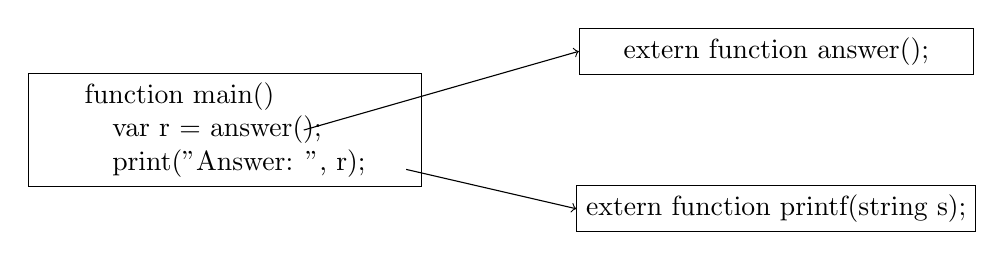
\begin{tikzpicture}[every text node part/.style={align=left}]
 \node [draw, minimum width=5cm] (main) { 
function main()\\
  \quad var r = answer(); \\
  \quad print("Answer: ", r);
};
 \node [draw, minimum width=5cm] (resp) at (7, 1) {extern function answer();};
 \node [draw, minimum width=5cm] (printf) at (7, -1) {extern function printf(string s);};

 \draw[->] (1,0) -- (resp.west);
 \draw[->] (2.3,-0.5) -- (printf.west);
\end{tikzpicture}
\end{center}

\end{frame}
%------------------------------------------------

\begin{frame}[fragile]{Link Time Optimization (LTO)}
\begin{itemize}
	\item Translation Unit callgraph of \texttt{b.c}
\end{itemize}

\begin{center}
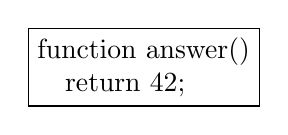
\begin{tikzpicture}[every text node part/.style={align=left}]
\centering
 \node [draw, minimum width=1cm] (main) { 
function answer()\\
  \quad return 42;
};
\end{tikzpicture}
\end{center}

\end{frame}

%------------------------------------------------

\begin{frame}[fragile]{Link Time Optimization (LTO)}

\begin{itemize}
    \item United Translation Unit callgraph with LTO
\end{itemize}

\begin{center}
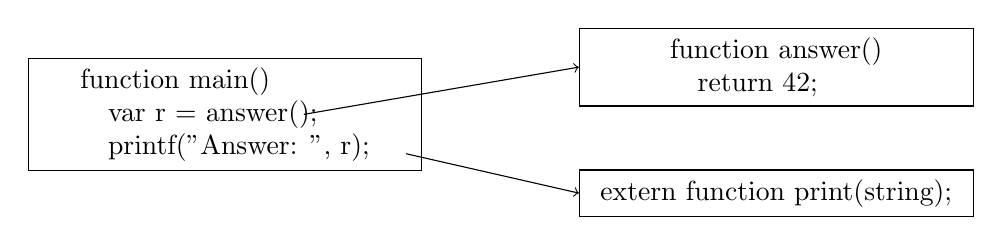
\begin{tikzpicture}[every text node part/.style={align=left}]
 \node [draw, minimum width=5cm] (main) { 
function main()\\
  \quad var r = answer(); \\
  \quad printf("Answer: ", r);
};
 \node [draw, minimum width=5cm] (resp) at (7, 0.6) {function answer()\\
 \quad return 42;
 };
 \node [draw, minimum width=5cm] (printf) at (7, -1) {extern function print(string);};

 \draw[->] (1,0) -- (resp.west);
 \draw[->] (2.3,-0.5) -- (printf.west);
\end{tikzpicture}
\end{center}

\begin{itemize}
	\item Now the compiler has enough information to inline \texttt{answer}
\end{itemize}

\end{frame}

%--------------------------------------------------------------------------------

\begin{frame}[fragile]{Link Time Optimization (LTO)}

\begin{itemize}
    \item LTO work in three stages: \cite{whoprgoogle,glek2010optimizing}
    \begin{itemize}
        \item LGEN (\textit{Local Generation}): Translate source to IR
        \item WPA (\textit{Whole Program Analysis}): Do analysis on callgraph
        \item LTRANS (\textit{Local Transformations}): Compile partitions to assembly
    \end{itemize}
\end{itemize}

\tikzstyle{block} = [rectangle, draw, fill=white,
    text width=6em, text centered, rounded corners, node distance=1cm and 0.5cm, minimum height=2em]
\tikzstyle{line} = [draw, -latex]
\makebox[\textwidth][c]{

\scalebox{0.5}{
\begin{tikzpicture}[node distance = 3cm, auto]
    % Place nodes
    \node [block]              (fonte1) {source1.c};
    \node [block, right= of fonte1]        (fonte2) {source2.cpp};
    \node [block, right= of fonte2]        (fonte3) {source3.f90};
    \node [block, above= of fonte2]         (make)   {Makefile};

    \node [block, below= of fonte1]        (gcc)      {gcc};
    \node [block, below= of fonte2]        (g++)      {g++};
    \node [block, below= of fonte3]        (gfortran) {gfortran};

    \node [block, below= of gcc]           (objeto1) {obj1.o};
    \node [block, below= of g++]           (objeto2) {obj2.o};
    \node [block, below= of gfortran]      (objeto3) {obj3.o};

    \node [block, below= of objeto2]       (gcc_lto) {collect2 (lto1)};

    \node [block, right= of fonte3]            (gcc_ltrans1) {gcc\_ltrans};
    \node [block, right= of gcc_ltrans1]   (gcc_ltrans2) {gcc\_ltrans};
    \node [block, right= of gcc_ltrans2]   (gcc_ltrans3) {gcc\_ltrans};

    \node [block, above= of gcc_ltrans2]       (gcc_wpa) {gcc\_wpa};
    \coordinate[below= of gcc_wpa]            (c2);


    \node [block, below= of gcc_ltrans1]   (obj1) {obj1.o};
    \node [block, below= of gcc_ltrans2]   (obj2) {obj2.o};
    \node [block, below= of gcc_ltrans3]   (obj3) {obj3.o};

    \node [block, below=of obj2]   (ld) {collect2 (LD)};

	\node [block, below=of ld]   (bin) {Binary};

    % Draw edges
    \draw[->]    ([xshift=-0.7em] make.south)   -- (fonte1.north);
    \draw[->]    (make.south)   -- (fonte2.north);
    \draw[->]    ([xshift=+0.7em] make.south)   -- (fonte3.north);

    \draw[->]    (fonte1.south)   -- (gcc.north);
    \draw[->]    (fonte2.south)   -- (g++.north);
    \draw[->]    (fonte3.south)   -- (gfortran.north);

    \draw[->]    (gcc.south)   -- (objeto1.north);
    \draw[->]    (g++.south)   -- (objeto2.north);
    \draw[->]    (gfortran.south)   -- (objeto3.north);

    \draw[->]    (objeto1.south)   -- ([xshift=-0.7em]gcc_lto.north);
    \draw[->]    (objeto2.south)   -- (gcc_lto.north);
    \draw[->]    (objeto3.south)   -- ([xshift=+0.7em]gcc_lto.north);

    %\draw[->]    (gcc_lto.south)   -- (gcc_wpa.north);
 	\draw[->]  (gcc_lto.east) .. controls +(7.5,0) and +(-7.5,0).. (gcc_wpa.west);

    \draw[->]    (gcc_wpa.south)   -- (gcc_ltrans1.north);
    \draw[->]    (gcc_wpa.south)   -- (gcc_ltrans2.north);
    \draw[->]    (gcc_wpa.south)   -- (gcc_ltrans3.north);

    \draw[->]    (gcc_ltrans1.south)   -- (obj1.north);
    \draw[->]    (gcc_ltrans2.south)   -- (obj2.north);
    \draw[->]    (gcc_ltrans3.south)   -- (obj3.north);

    \draw[->]    (obj1.south)   -- ([xshift=-0.7em]ld.north);
    \draw[->]    (obj2.south)   -- (ld.north);
    \draw[->]    (obj3.south)   -- ([xshift=+0.7em]ld.north);

	\draw[->]    (ld.south)   -- (bin.north);
	
	%draw brackets
\draw [decorate,decoration={brace,amplitude=10pt},xshift=-0.5cm,yshift=0pt]
([xshift=-1.3cm]objeto1.south) -- ([xshift=-1.3cm]fonte1.north) node [black,midway,xshift=-0.3cm]
{\footnotesize \begin{turn}{90}LGEN\end{turn}};

\draw [decorate,decoration={brace,amplitude=10pt},xshift=-0.5cm,yshift=0pt]
([xshift=1.3cm]gcc_ltrans3.north) -- ([xshift=1.3cm]obj3.south) node [black,midway,xshift=0.3cm]
{\footnotesize \begin{turn}{-90}LTRANS\end{turn}};


\draw [decorate,decoration={brace,amplitude=10pt},xshift=-0.5cm,yshift=0pt]
([xshift=1.3cm]gcc_wpa.north) -- ([xshift=1.3cm]gcc_wpa.south) node [black,midway,xshift=0.3cm]
{\footnotesize \begin{turn}{-90}WPA\end{turn}};


\end{tikzpicture}
}
}%

\end{frame}

%--------------------------------------------------------------------------------

\begin{frame}{Link Time Optimizations}

\begin{itemize}
    
    \item Refinements: Johnson \textit{et al.} \cite{thinlto} proposes ThinLTO
    \begin{itemize}
        \item Generate function summaries on LGEN
        \item Only uses summary on WPA stage to reduce memory usage
        \item Calculate function footprint to avoid recompiling the entire partition
    \end{itemize}
    \item[]

    \item Other approaches: Li \textit{et al.} \cite{lipo} proposes LIPO
    \begin{itemize}
        \item IPA analysis on binary runtime
        \item Load functions in other modules based on profiling report
    \end{itemize}
\end{itemize}

\end{frame}

%--------------------------------------------------------------------------------
\section{Proposed work}
%--------------------------------------------------------------------------------

\begin{frame}{Proposed work}

\begin{itemize}
    \item To compile source files in parallel:
    \begin{itemize}
        \item Parallelizing the compiler
        \item Which parts can be parallelized?
        \item[]
    \end{itemize}
    \item If we parallelize by functions:
    \begin{itemize}
        \item Intraprocedural Analysis can be easily parallelized
        \item Parser can be parallelized, as shown in Related Works
        \item Interprocedural Analysis: not trivial
    \end{itemize}
    \item Start tackling the most consuming part
\end{itemize}

\end{frame}

%--------------------------------------------------------------------------------

\begin{frame}{Proposed work}

\begin{itemize}
    \item To compile source files in parallel:
    \begin{itemize}
        \item Parallelizing the compiler
        \item Which parts can be parallelized?
        \item[]
    \end{itemize}
    \item If we parallelize by functions:
    \begin{itemize}
        \item Intraprocedural Analysis can be easily parallelized
        \item Parser can be parallelized, as shown in Related Works
        \item Interprocedural Analysis: not trivial
    \end{itemize}
    \item Start tackling the most consuming part
\end{itemize}
\end{frame}

%--------------------------------------------------------------------------------

\begin{frame}{Proposed work}
\begin{center}
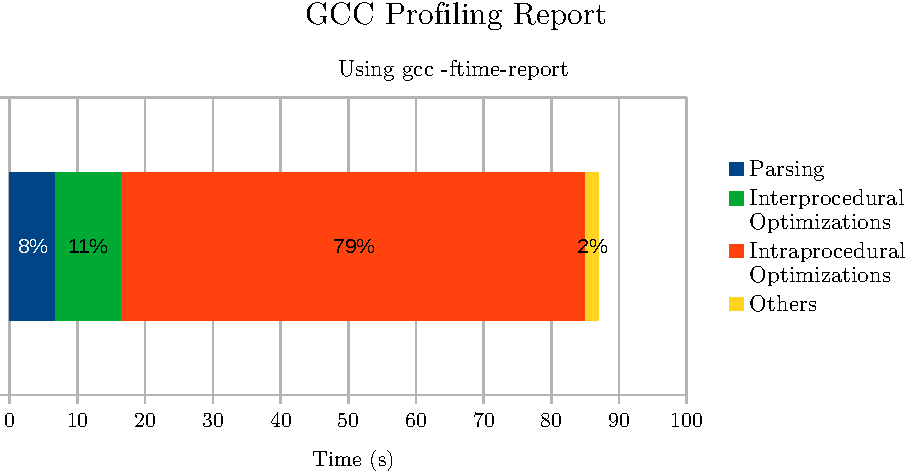
\includegraphics[scale=0.8]{figuras/profiling-crop.pdf}
\end{center}
\end{frame}

%--------------------------------------------------------------------------------

\begin{frame}{Proposed Work}

\begin{itemize}
    \item Intraprocedural Analysis take 79\% of compilation time
    \begin{itemize}
        \item Maximum speedup of $5\times$ if we parallelize only this part
        \item[]
    \end{itemize}
    \item We begin parallelizing Intraprocedural Analysis
    \begin{itemize}
        \item First attempt: threading the compiler
        \item Second attempt (succeded): partitioning the callgraph
    \end{itemize}
\end{itemize}
\end{frame}

%--------------------------------------------------------------------------------
\subsection{Parallelizing with threads}
%--------------------------------------------------------------------------------

\begin{frame}{Parallelizing with threads}

\begin{itemize}
    \item Idea: adapt work by Wortman and Junkin \cite{wortman1992}
    \begin{itemize}
        \item IPA output functions to a producer-consumer queue
        \item Intraprocedural Analyzer pop functions from this queue
        \item Barrier at code generation
        \item In GCC: Parallelize GIMPLE passes first, idea was move to RTL next
        \item[]
    \end{itemize}
 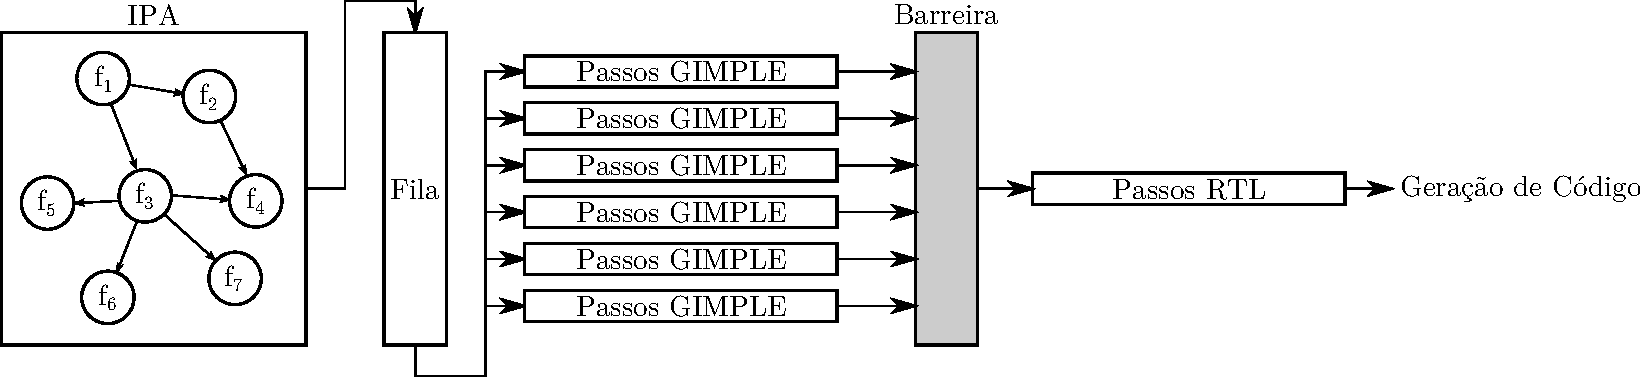
\includegraphics[scale=0.5]{paralelizacao.pdf}
\end{itemize}
\end{frame}

%--------------------------------------------------------------------------------

\begin{frame}{Parallelizing with threads}

\begin{itemize}
    \item Problems
    \begin{itemize}
        \item Garbage Collection (GC)
        \begin{itemize}
            \item Useful for holding tree nodes -- reference count
            \item Solution: use locks in the GC
        \end{itemize}
        \item Memory pools
        \begin{itemize}
            \item Seriallizing them made the compiler very slow
            \item Solution: Distributive approach, merge memory pools on request
        \end{itemize}
        \item Hash caches
        \begin{itemize}
            \item Use locks to ensure seriallize access
        \end{itemize}
        \item Target independent modules depending of Target dependent information
    \end{itemize}
\end{itemize}
\end{frame}

%--------------------------------------------------------------------------------

\begin{frame}{Parallelizing with threads}

\begin{itemize}
    \item Is this approach feasible?
    \begin{itemize}
        \item Yes, if we are building a compiler from the ground up
        \item No, if we are working on legacy code -- classical race condition problems
        \begin{itemize}
            \item Race condition detectors failing to detect race conditions
            \item Hard to track down the cause of issue
            \item Hard to test modifications incrementally
            \item Hard to ensure that builds are reproducible
        \end{itemize}
    \end{itemize}
\end{itemize}
\end{frame}

%--------------------------------------------------------------------------------

\begin{frame}{Parallelizing with threads}

\begin{itemize}
    \item 
    \begin{itemize}
        \item Yes, if we are building a compiler from the ground up
        \item No, if we are working on legacy code -- classical race condition problems
        \begin{itemize}
            \item Race condition detectors failing to detect race conditions
            \item Hard to track down the cause of issue
            \item Hard to test modifications incrementally
            \item Hard to ensure that builds are reproducible
        \end{itemize}
    \end{itemize}
\end{itemize}
\end{frame}

%--------------------------------------------------------------------------------

\begin{frame}{Parallelizing with threads}

\begin{itemize}
    \item Results
\end{itemize}
\begin{columns}
\begin{column}{0.5\textwidth}
 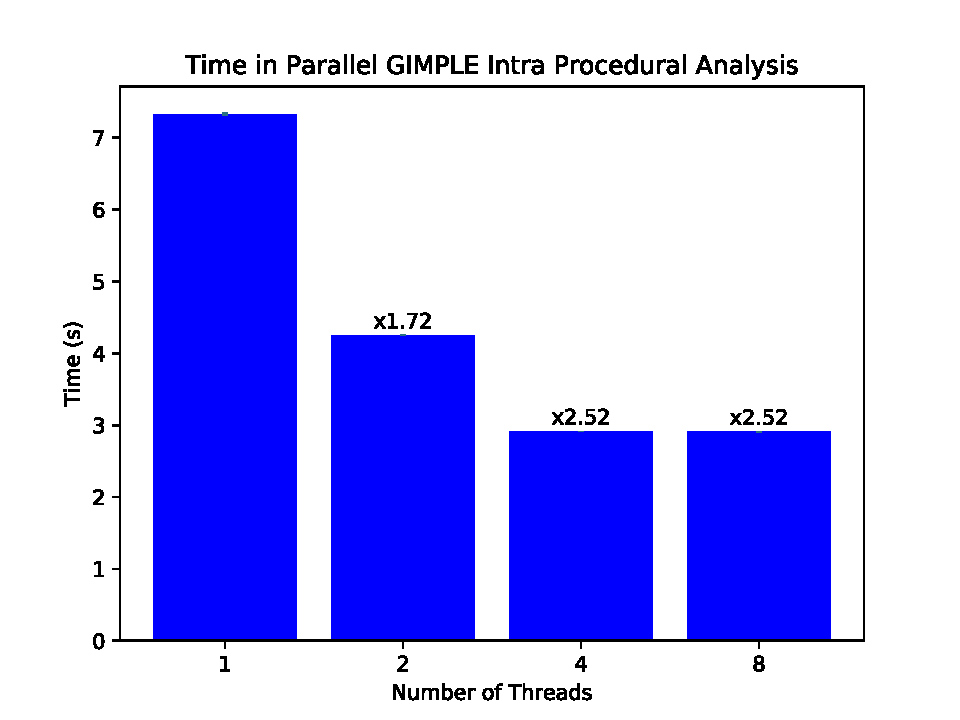
\includegraphics[scale=0.4]{gimple_parallel.pdf}
\end{column}
\begin{column}{0.5\textwidth}
 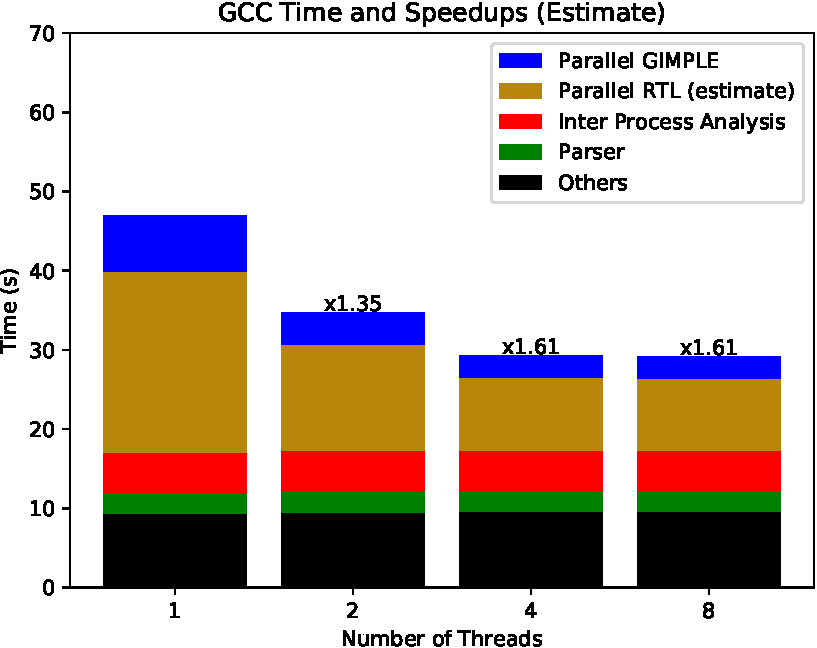
\includegraphics[scale=0.4]{gcc_estimate.pdf}
\end{column}
\end{columns}
\begin{itemize}
    \item Up to $2.52\times$ on GIMPLE, $1.61\times$ total in compiler
\end{itemize}

\end{frame}

%--------------------------------------------------------------------------------
\subsection{Parallelizing by partitioning the callgraph}
%--------------------------------------------------------------------------------

\begin{frame}{Parallelizing by partitioning the callgraph}

\begin{itemize}
    \item Idea: Reuse the largely serial and tested parts of the compiler
    \item Callgraph partitioning is already implemented in LTO
    \begin{itemize}
        \item Can we modify it to compile a single file?
    \end{itemize}
\end{itemize}
\end{frame}

%--------------------------------------------------------------------------------

\begin{frame}{Parallelizing by partitioning the callgraph}

\begin{itemize}
    \item First part: ensure that the partitioned code will be merged together 
    \begin{itemize}
        \item Generate a single object file for each partition
        \item Link them together using partial linking
    \end{itemize}
\end{itemize}

\tikzstyle{block} = [rectangle, draw, fill=white,
    text width=6em, text centered, rounded corners, minimum height=2em]
\tikzstyle{line} = [draw, -latex]

\makebox[\textwidth][c]{
\scalebox{0.6}{
\begin{tikzpicture}[node distance = 3cm, auto]
    % Place nodes
    \node [block]                      (cc1_1) {cc1};
    \coordinate [right= of cc1]          (c);
    \node [block, right= of c,fill={rgb:black,1;white,2}]        (driver1) {gcc};
    \node [block, above= of c]                      (cc1_2) {cc1};
    \node [block, below= of c]                      (cc1_3) {cc1};
    \coordinate [above= of driver1]          (c2);
    \coordinate [below= of driver1]          (c3);
    \node [block, right= of c2]      (as2) {as};
    \node [block, right= of c3]      (as3) {as};
    \node [block, right= of driver1]       (ld) {ld};
    \coordinate [left= of cc1]          (fonte);
    \coordinate [right= of ld]    (bin);

    % Draw edges
    \draw[->]    (driver1.west)    -- (cc1_1.east) node[midway, above] {\texttt{-fadditional-asm=<file>}};
    \draw[->]    ([xshift=+0.5cm]cc1_2.south) -- ([xshift=-0.5cm]driver1.north) node[midway, above, sloped] {Generates .s file};
    \draw[->]    ([xshift=+0.5cm]cc1_3.north) -- ([xshift=-0.5cm]driver1.south) node[midway, above, sloped] {Generates .s file};

    \draw[->]    (cc1_1.north)    -- ([xshift=-0.5cm]cc1_2.south) node[midway, above, sloped] {Forks};
    \draw[->]    (cc1_1.south)    -- ([xshift=-0.5cm]cc1_3.north) node[midway, above, sloped] {Forks};

    \draw[->]    ([xshift=+0.5cm]driver1.north)  -- (as2.south) node[midway, above, sloped] {Assemble received .s};
    \draw[->]    ([xshift=+0.5cm]driver1.south)  -- (as3.north) node[midway, above, sloped] {Assemble receibed .s};
    \draw[->]    (driver1.east)  -- (ld.west) node[midway, above, sloped] {Links};

%    \draw[->]    (cc1.east)    -- (as.west)       node[midway, above] {Assembler File};
%    \draw[->]    (cc1.east)    -- (as.west)       node[midway, above] {Assembler File};
%
%    \draw[->]    (cc1.east)    -- (as.west)       node[midway, below] {(.s)};
    \draw[->]    ([xshift=+0.5cm]as2.south)     -- (ld.north)       node[midway, above, sloped] {Object File};
    \draw[->]    ([xshift=+0.5cm]as3.north)     -- (ld.south)       node[midway, below, sloped] {Object File};
%    \draw[->]    (fonte.west)  -- (cc1.west)      node[pos=0, above] {Source File};
%    \draw[->]    (fonte.west)  -- (cc1.west)      node[pos=0, below] {(.c)};
    \draw[->]    (ld.east)     -- (bin.west)      node[pos=1, above] {\texttt{file.o}};
\end{tikzpicture}
}
}
\end{frame}

%--------------------------------------------------------------------------------

\begin{frame}{Parallelizing by partitioning the callgraph}

\begin{itemize}
    \item Adapting the LTO Partitioner:
    \begin{itemize}
        \item Find all dependencies: COMDAT groups
        \item Propagate to all symbols touching the COMDAT group
        \item Agglutinate to the same partition
    \end{itemize}
\begin{center}
	 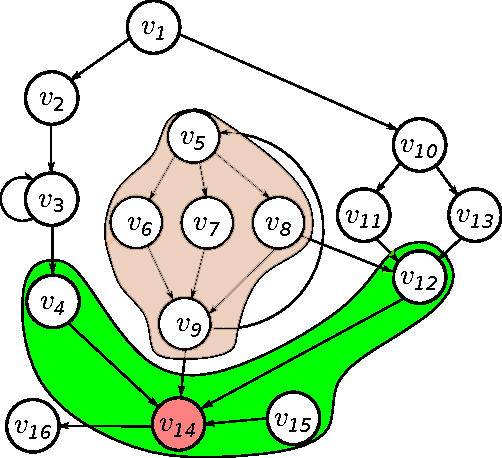
\includegraphics[scale=0.5]{figuras/comdat_frontier.pdf}
\end{center}
\end{itemize}
\end{frame}

%--------------------------------------------------------------------------------

\begin{frame}{Parallelizing by partitioning the callgraph}

\begin{itemize}
    \item Boundary Computation
    \begin{itemize}
        \item Add functions and variables referenced in the partition
        \item Remove the body of functions in boundary
        \item Avoid removing if function is marked to be inlined
        \item Promote private function in boundary to global
        \begin{itemize}
            \item Mangle names to avoid clashing
        \end{itemize}
    \end{itemize}
    \item Partition application can be reduced to four cases:
    \begin{itemize}
        \item \textit{Node is in partition}
        \item \textit{Node is in boundary, but keeping its body}
        \item \textit{Node is in boundary}
        \item \textit{Node not in boundary}
    \end{itemize}
    \item Communicate the partition number to the driver
\end{itemize}
\end{frame}

%--------------------------------------------------------------------------------

\begin{frame}{Parallelizing by partitioning the callgraph}

\begin{itemize}
    \item Builds are reproducible
    \begin{itemize}
        \item No random information is necessary to solve name clashing
        \item Always generate the same partitions
        \item Partial Linking is always done in the same order
        \item No other race conditions are introduced
    \end{itemize}
\end{itemize}
\end{frame}

\begin{frame}{Parallelizing by partitioning the callgraph}
\begin{itemize}
    \item Results
    \item[]

\begin{center}
\resizebox{.9\textwidth}{!}{%
\begin{tabular}{|l|c|c|c|c|}
\hline
File             & Sequential & 8 Threads & Speedup      & \multicolumn{1}{l|}{Sequential} \\ \hline
gimple-match.c   & $76s$      & $31s$     & $2.4\times$  & $221s$                          \\ \hline
insn-emit.c      & $23s$      & $10s$     & $2.25\times$ & $97s$                           \\ \hline
tree-vect-stmt.c & $11s$      & $5s$      & $2.14\times$ & $32s$                           \\ \hline
brig-lang.c      & $10s$      & $15s$     & $0.7\times$  & $29s$                           \\ \hline
\end{tabular}
}
\end{center}
\end{itemize}
\end{frame}

%--------------------------------------------------------------------------------

\begin{frame}{Parallelizing by partitioning the callgraph}

\begin{itemize}
    \item Feasibilty
    \begin{itemize}
        \item Quick to implement
        \item Rely on tested serial parts of the compiler
        \item No other race conditions are introduced
    \end{itemize}
\end{itemize}
\end{frame}

%--------------------------------------------------------------------------------

\begin{frame}{Parallelizing by partitioning the callgraph}
\begin{itemize}
    \item Results
    \item[]

\begin{center}
\resizebox{.9\textwidth}{!}{%
\begin{tabular}{|l|c|c|c|c|}
\hline
File             & Sequential & 8 Threads & Speedup      & \multicolumn{1}{l|}{Sequential} \\ \hline
gimple-match.c   & $76s$      & $31s$     & $2.4\times$  & $221s$                          \\ \hline
insn-emit.c      & $23s$      & $10s$     & $2.25\times$ & $97s$                           \\ \hline
tree-vect-stmt.c & $11s$      & $5s$      & $2.14\times$ & $32s$                           \\ \hline
\end{tabular}
}
\end{center}
\end{itemize}
\end{frame}

%--------------------------------------------------------------------------------
\section{Experiments and Results}
%--------------------------------------------------------------------------------

\begin{frame}{Experiments}

\begin{itemize}
    \item Two machines:
    \begin{itemize}
        \item Core-i7: 8 threads, 4 cores CPU
        \item Optreon 6376: 64 threads, 32 cores CPU
    \end{itemize}
    \item Partitioning quota:
    \begin{itemize}
        \item Minimum program size to start partitioning
        \item $10^3$ and $10^5$
    \end{itemize}
    \item 15 samples per file, 5 samples per project
\end{itemize}
\end{frame}

%--------------------------------------------------------------------------------

\begin{frame}{Experiments}
\resizebox{\textwidth}{!}{%
\begin{tabular}{l|c|c|c|c|c|c|c|c}
\cline{2-7}
                                       & \multicolumn{3}{c|}{Core-i7}     & \multicolumn{3}{c|}{Opteron 6376}                                                                & \multicolumn{1}{l}{}               \\ \hline
\multicolumn{1}{|l|}{File}             & Sequential & 8 Threads & Speedup & \multicolumn{1}{l|}{Sequential} & \multicolumn{1}{l|}{64 Threads} & \multicolumn{1}{l|}{Speedup} & \multicolumn{1}{c|}{Autogenerated} & \multicolumn{1}{c|}{LoC}  \\ \hline
\multicolumn{1}{|l|}{gimple-match.c}   & $76s$        & $31s$       & $2.4\times$     & $221s$                            & $66s$                             & $3.32\times$                         & \multicolumn{1}{c|}{yes} & \multicolumn{1}{c|}{$244320$}          \\ \hline
\multicolumn{1}{|l|}{insn-emit.c}      & $23s$        & $10s$       & $2.25\times$    & $97s$                             & $37s$                             & $3.53\times$                         & \multicolumn{1}{c|}{yes}  & \multicolumn{1}{c|}{$273482$}         \\ \hline
\multicolumn{1}{|l|}{tree-vect-stmt.c} & $11s$        & $5s$        & $2.14\times$    & $32s$                             & $13s$                             & $2.46\times$                         & \multicolumn{1}{c|}{no}    & \multicolumn{1}{c|}{$12133$}        \\ \hline
\multicolumn{1}{|l|}{brig-lang.c} & $11s$        & $11	s$        & $1.02\times$    & $29s$                             & $29s$                             & $1.02\times$                         & \multicolumn{1}{c|}{no}    & \multicolumn{1}{c|}{$958$}        \\ \hline
\end{tabular}
}
\end{frame}


%--------------------------------------------------------------------------------

\begin{frame}{Experiments}
\resizebox{\textwidth}{!}{%
\begin{tabular}{l|c|c|c|c|c|c|c|c}
\cline{2-7}
                                       & \multicolumn{3}{c|}{Core-i7}     & \multicolumn{3}{c|}{Opteron 6376}                                                                & \multicolumn{1}{l}{}               \\ \hline
\multicolumn{1}{|l|}{File}             & Sequential & 8 Threads & Speedup & \multicolumn{1}{l|}{Sequential} & \multicolumn{1}{l|}{64 Threads} & \multicolumn{1}{l|}{Speedup} & \multicolumn{1}{c|}{Autogenerated} & \multicolumn{1}{c|}{LoC}  \\ \hline
\multicolumn{1}{|l|}{gimple-match.c}   & $76s$        & $31s$       & $2.4\times$     & $221s$                            & $66s$                             & $3.32\times$                         & \multicolumn{1}{c|}{yes} & \multicolumn{1}{c|}{$244320$}          \\ \hline
\multicolumn{1}{|l|}{insn-emit.c}      & $23s$        & $10s$       & $2.25\times$    & $97s$                             & $37s$                             & $3.53\times$                         & \multicolumn{1}{c|}{yes}  & \multicolumn{1}{c|}{$273482$}         \\ \hline
\multicolumn{1}{|l|}{tree-vect-stmt.c} & $11s$        & $5s$        & $2.14\times$    & $32s$                             & $13s$                             & $2.46\times$                         & \multicolumn{1}{c|}{no}    & \multicolumn{1}{c|}{$12133$}        \\ \hline
\multicolumn{1}{|l|}{{\color{red} brig-lang.c}} & $11s$        & $11	s$        & {\color{red}$1.02\times$}    & $29s$                             & $29s$                             & $1.02\times$                         & \multicolumn{1}{c|}{no}    & \multicolumn{1}{c|}{$958$}        \\ \hline
\end{tabular}
}
\end{frame}

%--------------------------------------------------------------------------------
\begin{frame}[fragile]{Experiments}
\begin{columns}
\begin{column}{0.5\textwidth}

\begin{verbatim}
Num threads: 8
Promote priv. functions: true
Without debug symbols
Wall clock time: 11.083s
Phases:
  Parsing: 1.145s
  IPA: 1.885s
  Partitioner: 0.003s
  LTRANS: 9.849s
\end{verbatim}

\end{column}


\begin{column}{0.5\textwidth}
\begin{verbatim}
Num threads: 1
Promote priv. functions: true
Without debug symbols
Wall clock time: 11.383s
Phases:
  Parsing: 2.1498s
  IPA: 1.916s
  Intraprocedural: 8.868s
\end{verbatim}
\end{column}
\end{columns}
\end{frame}

%--------------------------------------------------------------------------------
\begin{frame}[fragile]{Experiments}
\begin{verbatim}
Number of partitions: 2
Partition: 0, Nr of insns: 4465, Symbols: 483
  ...

Partition: 1, Nr of insns: 51356, Symbols: 2842
  ...
  Node name: brig_define_builtins, insns: 47261
\end{verbatim}
\begin{itemize}
    \item $84\%$ of generated code belongs to a single function
\end{itemize}

\end{frame}

%--------------------------------------------------------------------------------

\begin{frame}[fragile]{Experiments}
\begin{itemize}
    \item Effect on projects:
    \begin{itemize}
        \item Up to 35\% improvement
    \end{itemize}

\end{itemize}
\begin{center}
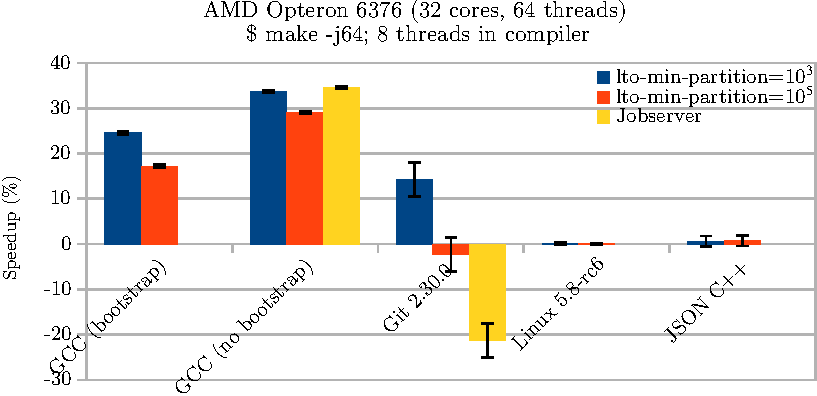
\includegraphics[scale=0.7]{figuras/experiment_projects_new-crop.pdf}
\end{center}
\end{frame}

%--------------------------------------------------------------------------------

\begin{frame}{Experiments}
\begin{itemize}
    \item Compiling GCC without our changes
\end{itemize}
\begin{center}
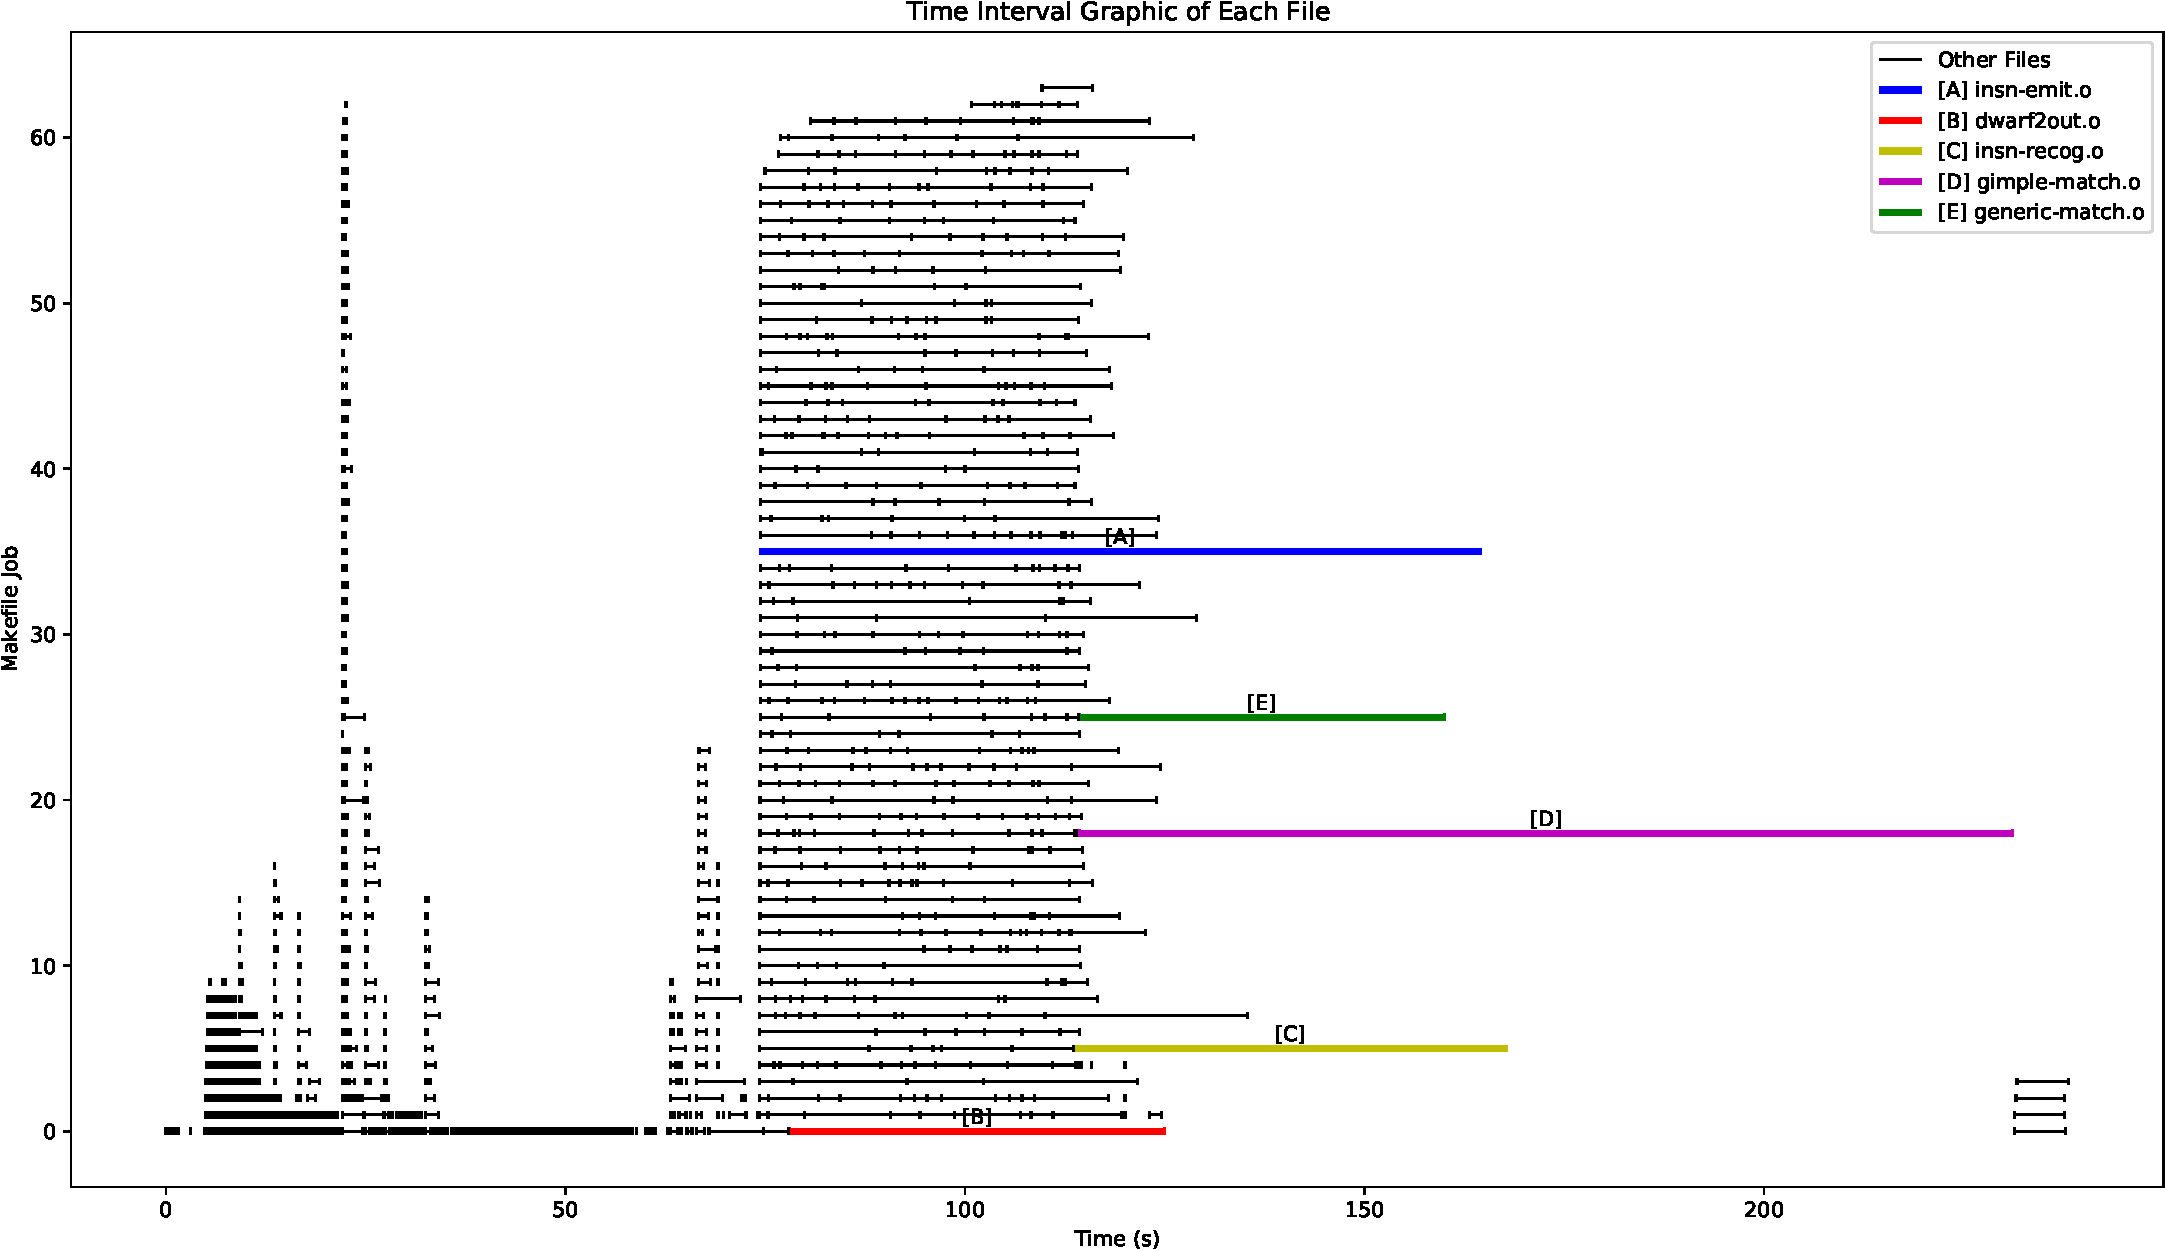
\includegraphics[scale=.3]{seq-crop.pdf}
\end{center}
\end{frame}

%--------------------------------------------------------------------------------

\begin{frame}[fragile]{Experiments}
\begin{itemize}
    \item Compiling GCC with our changes
\end{itemize}
\begin{center}
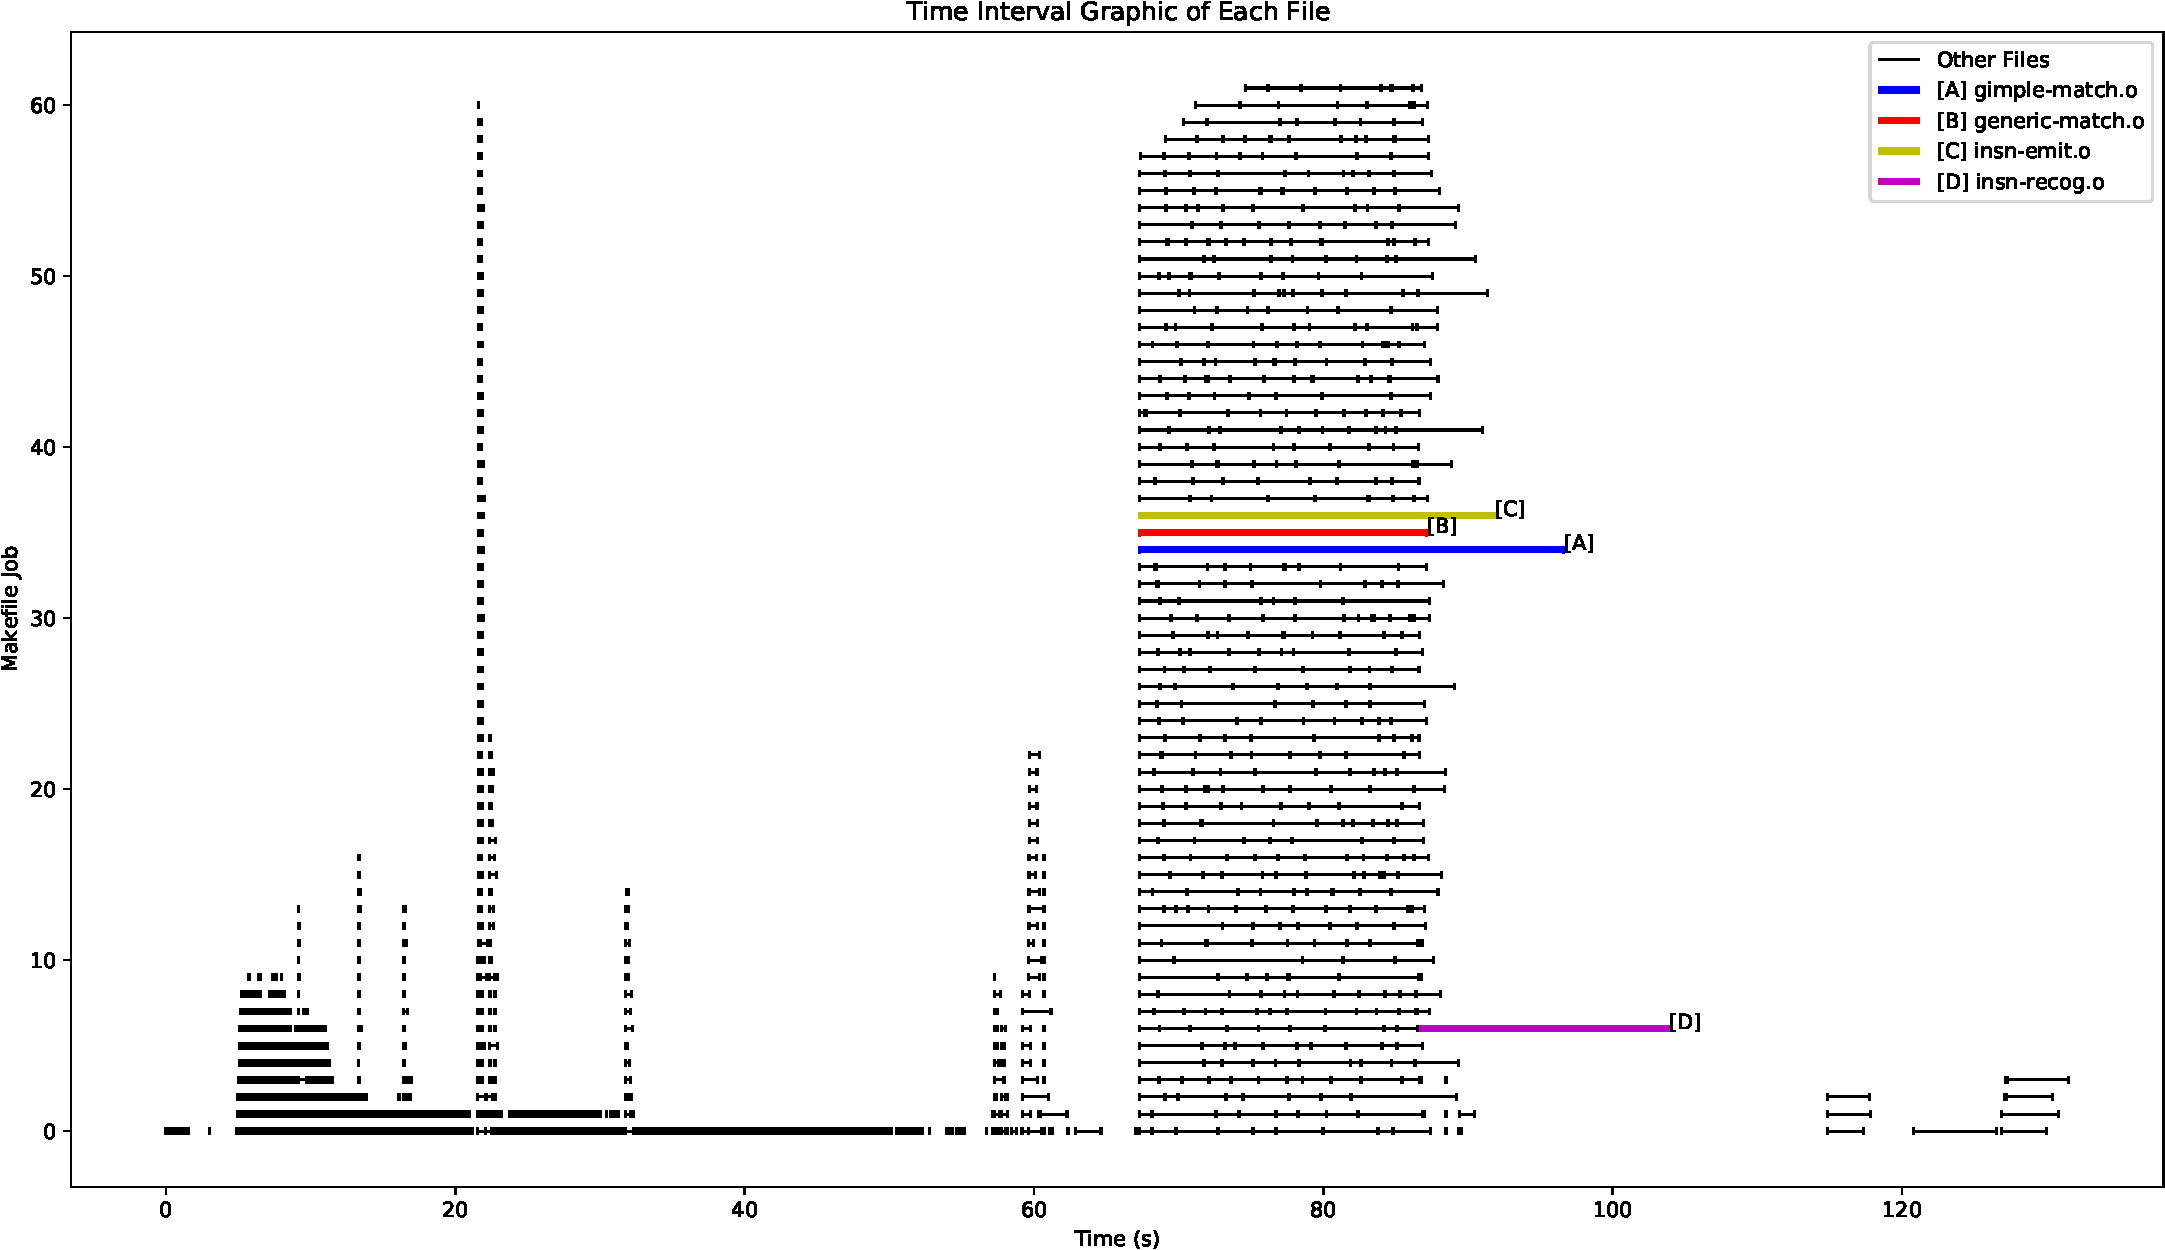
\includegraphics[scale=.3]{par-crop.pdf}
\end{center}
\end{frame}

%--------------------------------------------------------------------------------

\begin{frame}{Experiments}
\begin{itemize}
    \item Power consumption measurement
\end{itemize}
\begin{center}
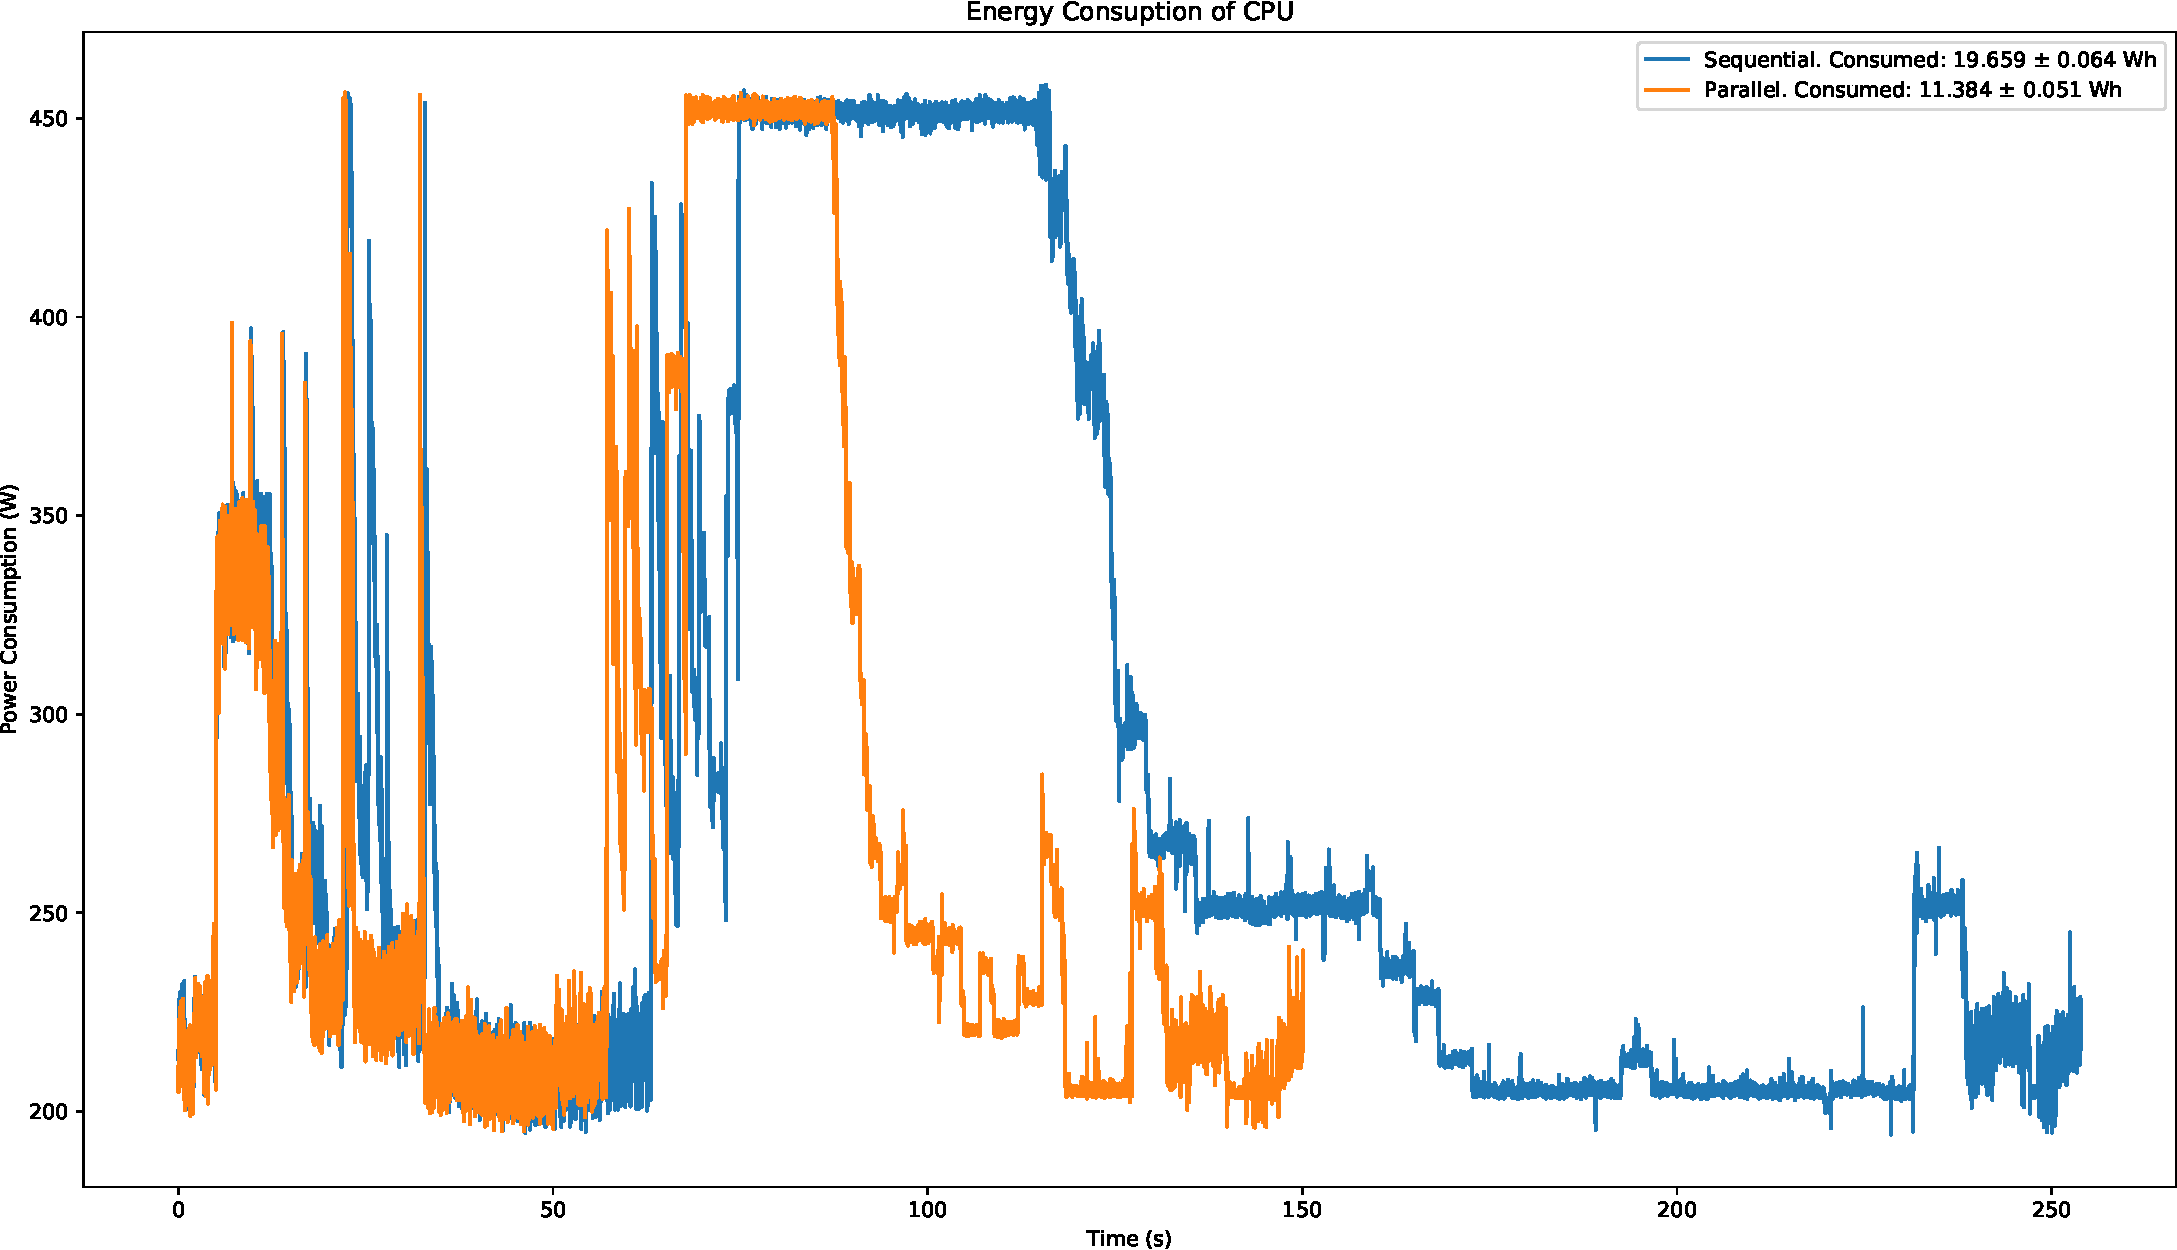
\includegraphics[scale=.3]{power-crop.pdf}
\end{center}
\end{frame}

%--------------------------------------------------------------------------------
\section{Conclusions}
%--------------------------------------------------------------------------------

\begin{frame}{Conclusions}
\begin{itemize}
    \item We presented a method of parallelizing a significant part of a compiler
    \begin{itemize}
        \item Intraprocedural Analysis consume large amount of time
        \item Reuse the LTO engine to incrementally parallelize compilation
    \end{itemize}
    \item[]
    \item RQ1 - Main point that can take advantage of parallelism
    \begin{itemize}
        \item Intraprocedural Analysis
        \item Takes $79\%$ of runtime
    \end{itemize}
\end{itemize}
\end{frame}

%--------------------------------------------------------------------------------

\begin{frame}{Conclusions}
\begin{itemize}
    \item RQ2 - Performance improvement
    \begin{itemize}
        \item Up to $3.52\times$ when compiling individual files
        \item Up to $35\%$ when compiling projects
    \end{itemize}
    \item[]
    \item RQ3 - When is compiling in parallel faster
    \begin{itemize}
        \item Existence of blob files
        \begin{itemize}
            \item Takes significant amount of time when compared to remaining files
        \end{itemize}
        \item Not enough files to populate the CPU
    \end{itemize}
    \item RQ4 - How does it impact consumption
    \begin{itemize}
        \item Reduction of $8.27Wh$ of power consumption when compiling GCC
        \item Better usage of cores $\rightarrow$ less power consumption
    \end{itemize}
\end{itemize}
\end{frame}

%--------------------------------------------------------------------------------

\begin{frame}{Conclusions}
\begin{itemize}
    \item Future Works
    \begin{itemize}
        \item Develop a predictive model to automatically decide to run in parallel
        \item Improve our partitioner algorithm
        \item Avoid relying on partial linking
        \item Research about how to parallelize Interprocedural Optimizations
    \end{itemize}
\end{itemize}
\end{frame}

%--------------------------------------------------------------------------------

\begin{frame}{Thank you!}
\begin{center}
    \huge Thank you!
\end{center}
\end{frame}


%\begin{frame}{Parallelization by partitioning the callgraph}
%  \begin{columns}[t]
%    \col
%      \begin{coloredblock}{red!90!black}{Functional requirements}
%        \begin{itemize}
%          \item Integration and Management of IoT Devices
%          \item Data Acquisition, Storing, and Processing
%          \item Context-awareness
%          \item City Resource Discovery
%          \item Geolocation-based Services
%          \item External data access
%        \end{itemize}
%      \end{coloredblock}
%
%    \col
%      \begin{coloredblock}{red!90!black}{Non-functional requirements}
%        \begin{itemize}
%          \item Interoperability
%          \item Scalability
%          \item Security
%          \item Privacy
%          \item Evolvability
%          \item Adaptability
%        \end{itemize}
%      \end{coloredblock}
%  \end{columns}
%\end{frame}
%
%\begin{frame}{Theorems and proofs}
%  \pause
%  \begin{theorem}[An example theorem]
%    Theorem\dots
%  \end{theorem}
%
%  \pause
%  \begin{example}[An example of an example]
%    Example\dots
%  \end{example}
%
%  \pause
%  \begin{proof}[An example proof]
%    Proof\dots
%  \end{proof}
%
%  \pause
%  \begin{definition}[An example definition]
%    Definition\dots
%  \end{definition}
%
%  \pause
%  \begin{proposition}[An example proposition]
%    Proposition\dots
%  \end{proposition}
%\end{frame}
%
%\section{Related Works}
%
%\begin{frame}{Related Works}
%\end{frame}
%
%\section{Methodology}
%
%\begin{frame}{Methodology}
%\end{frame}
%
%\section{Results}
%
%\subsection{Validation and Analysis}
%
%\begin{frame}{Validation}
%\end{frame}
%
%\begin{frame}{Case Study}
%\end{frame}
%
%\section{Conclusion and Future works}
%
%\begin{frame}{Conclusion and Future works}
%\end{frame}

\section{References}

\begin{frame}[allowframebreaks]{References}
  \nocite{bronevetsky02, schmidt03:MSc, FSF:GNU-GPL, CORBA:spec, MenaChalco08, natbib, biblatex, eco:09}
  \printbibliography
\end{frame}

% Recapitulando
\begin{frame}{\insertshorttitle}
  \overview

  % \begin{center} acrescenta espaço vertical;
  % como possivelmente temos bem pouco espaço aqui,
  % vamos usar centering
  {%
    \centering\noindent%
    \url{https://gitlab.com/link-of-your-repository}\par
  }

\end{frame}

%\showqrcode

%\appendix

%\begin{frame}{Extra info}
%  \begin{itemize}
%    \item It is often useful to have some extra slides addressing likely questions from the audience at the end of the presentation
%    \item By putting them after the ``appendix'' command, they are not counted in the page count indicator
%  \end{itemize}
%\end{frame}
%
%

%\providecommand\aviso[1]{
  \clearpage
  \null
  \vfill
  \begin{hyphenrules}{nohyphenation}
    \centering\bfseries\Large
    #1\par
  \end{hyphenrules}
  \vfill
  \clearpage
}

\providecommand\avisoFolhasDeRosto{
  \aviso{
    {\huge Você precisa editar os arquivos no diretório ``\texttt{conteudo}''!}
    \par\bigskip\bigskip\bigskip\bigskip
    Para gerar a capa e demais páginas preliminares no formato correto,
    modifique os arquivos ``\texttt{conteudo/paginas-preliminares.tex}'' e
    ``\texttt{conteudo/metadados.tex}'', usando como base os arquivos
    correspondentes no diretório ``\texttt{conteudo-exemplo}''.
  }
}

\providecommand\avisoCapitulos{
  \aviso{
    Insira o conteúdo dos capítulos do seu trabalho no arquivo
    ``\texttt{capitulos.tex}'' do diretório ``\texttt{conteudo}''.
  }
}

\providecommand\avisoApendices{
  \aviso{
    Insira o conteúdo dos apêndices do seu trabalho no arquivo
    ``\texttt{apendices.tex}'' do diretório ``\texttt{conteudo}''.
  }
}

\providecommand\avisoAnexos{
  \aviso{
    Insira o conteúdo dos anexos do seu trabalho no arquivo
    ``\texttt{anexos.tex}'' do diretório ``\texttt{conteudo}''.
  }
}

\providecommand\avisoArtigo{
  \aviso{
    Insira o conteúdo do artigo no arquivo ``\texttt{corpo-artigo.tex}''
    do diretório ``\texttt{conteudo}''. Não se esqueça de consultar
    o exemplo no diretório ``\texttt{conteudo-exemplo}'' para a
    definição do título, autoria etc.
  }
}

\providecommand\avisoApresentacao{
  \begin{frame}{Insira o conteúdo!}
  \aviso{
    Insira o conteúdo da apresentação no arquivo ``\texttt{corpo-apresentacao.tex}''
    do diretório ``\texttt{conteudo}''. Não se esqueça de consultar
    o exemplo no diretório ``\texttt{conteudo-exemplo}'' para a
    definição do título, autoria, estrutura etc.
  }
  \end{frame}
}

\providecommand\avisoPoster{
  \aviso{
    Insira o conteúdo do poster no arquivo ``\texttt{corpo-poster.tex}''
    do diretório ``\texttt{conteudo}''. Não se esqueça de consultar
    o exemplo no diretório ``\texttt{conteudo-exemplo}'' para a
    definição do título, autoria, estrutura etc.
  }
}

%\avisoApresentacao
